\begin{beginningnote}
    Al fine di evitare incomprensioni relative alla terminologia usata all’interno del presente documento, viene fornito un Glossario di progetto. Ogni terminologia specifica di progetto verrà chiarita e definita in modo tale da renderla maggiornamente comprensibile ed evitare errate interpretazioni. Pertanto ogni termine marchiato con una lettera \textbf{G} come apice, sarà specificato e presente nel glossario sopra citato.
\end{beginningnote}

%%%%%%%%%%%%%%%%%%%%%%%%%%%%%%%%%%%
% SCOPO DEL DOCUMENTO
%%%%%%%%%%%%%%%%%%%%%%%%%%%%%%%%%%%
\section{Scopo del Documento}\label{sec:scopo_del_documento}
Il presente documento ha lo scopo di fornire una descrizione dettagliata dei requisiti di progetto. Il documento è quindi frutto di un'attenta analisi del capitolato, proposto dal proponente, al fine di individuare ed esaminare in modo esaustivo i requisiti minimi, massimi e facoltativi presenti nel progetto. 
Un ulteriore obbiettivo del documento è quello di analizzare e descrivere le possibili attività (use cases) permesse all'utente in fase di esecuzione del programma. 

%%%%%%%%%%%%%%%%%%%%%%%%%%%%%%%%%%%
% IL PROGETTO
%%%%%%%%%%%%%%%%%%%%%%%%%%%%%%%%%%%
\section{Il progetto}\label{sec:progetto}
\subsection{Scopo del progetto}\label{sec:scopo_del_progetto}
Lo scopo del progetto è quello di ottimizzare i processi produttivi attraverso l'utilizzo di 
un applicativo 3D che rappresenta lo stato di fatto di un magazzino di stoccaggio.\\
L'applicativo, pensato per un utilizzo da ufficio (di tipo amministrativo), deve permettere all'utente di muoversi all'interno 
del magazzino e poter gestire le seguenti operazioni:
\begin{itemize}
    \item Creazione magazzino:
        \begin{itemize}
            \item Creare un nuovo magazzino da zero
            \item Importare un layout esistente
        \end{itemize}
    \item Modifiche alla struttura del magazzino:
        \begin{itemize}            
            \item Aggiungere nuove scaffalature
            \item Rimuovere scaffalature esistenti
            \item Modificare scaffalature
        \end{itemize}
    \item Modifiche ai prodotti presenti in magazzino:
        \begin{itemize}            
            \item Aggiungere un nuovo prodotto
            \item Eliminare un prodotto
            \item Spostare un prodotto esistente
        \end{itemize}
\end{itemize}
Si vuole sfruttare l'esperienza tridimensionale per aiutare la comprensione e facilitare la gestione delle 
operazioni di logistica necessarie sopra elencate. 


\subsection{Descrizione del prodotto}\label{sec:descrizione_del_prodotto}
L'applicativo, pensato per soddisfare lo scopo e i requisiti di progetto, si compone principalmente di due sezioni:
\begin{itemize}
    \item La prima sezione consente all'utente di interagire con il magazzino, per effettuare operazioni che ne vanno a modificare lo stato attuale (e.g. inserimento e modifica di scaffalature/prodotti, richieste di movimentazione);
    \item La seconda parte invece è composta dalla visualizzazione vera e propria del magazzino 3D. In questa area l'utente avrà modo di ``navigare" il magazzino. 
\end{itemize}

\newpage
%%%%%%%%%%%%%%%%%%%%%%%%%%%%%%%%%%%
% USE CASES
%%%%%%%%%%%%%%%%%%%%%%%%%%%%%%%%%%%
\section{Use Cases}\label{sec:use_cases}

\subsection{Attori}\label{subsec:attori}
Come da specifiche del proponente (si veda \ref{sec:riferimenti_normativi} per il link al capitolato), interessano soltanto sessioni volatili e con la sola gestione ``amministratore”. Pertanto, non sarà necessaria alcuna autenticazione nell'applicazione nè saranno presenti diverse tipologie di utenti con permessi distinti. L'unico attore\textsuperscript{G}, capace di accedere a tutte le funzionalità dell'applicazione e protagonista di tutti i casi d'uso, sarà dunque un utente generico amministratore, denominato \textbf{User}.

\subsection{Elenco dei casi d'uso}\label{subsec:elenco_use_cases}
\setcounter{secnumdepth}{0}         %per non mostrare numeri sezioni su indice
\subsection{UC1 - Creazione Magazzino}
\begin{figure}[H]
    \centering
    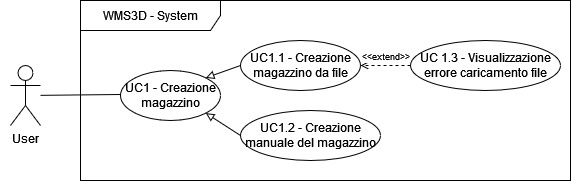
\includegraphics[width=0.8\textwidth]{UC_diagrams_1-10/UC1_sys.drawio.png}
    \caption{Diagramma UML UC1 - Creazione Magazzino}
\end{figure}
\begin{itemize}
    \item \textbf{Attori:} User.
    \item \textbf{Pre-condizione:} L'applicazione è avviata e funzionante.
    \item \textbf{Post-condizione:} Il magazzino viene creato e potrà essere visualizzato.
    \item \textbf{Scenario Principale:}  L’utente accede al sistema e sceglie una modalità di costruzione o attraverso file [UC1.1] o manualmente [UC1.2]. I dati necessari sono poi inseriti correttamente dall'utente e il magazzino viene costruito.
    \item \textbf{Generalizzazioni:} Sono presenti due generalizzazioni: 
    \begin{itemize}
        \item UC1.1 - Creazione magazzino tramite file;
        \item UC1.2 - Creazione manuale del magazzino.
    \end{itemize}
    \item \textbf{Estensioni:} -
\end{itemize}


\subsubsection{UC1.1 - Creazione magazzino da file}
\begin{itemize}
    \item \textbf{Attori:} User.
    \item \textbf{Pre-condizione:} L'applicazione è avviata e funzionante e l'utente dispone di un file contenente tutti i dati di costruzione di un magazzino 3D.
    \item \textbf{Post-condizione:} I dati vengono caricati correttamente e il magazzino viene creato e potrà essere visualizzato.
    \item \textbf{Scenario Principale:}  L’utente accede al sistema e sceglie la modalità di costruzione attraverso file. Procede dunque al caricamento dei dati tramite file e il magazzino viene costruito.
    \item \textbf{Generalizzazioni:} -
    \item \textbf{Estensioni:} È presente una estensione:
    \begin{itemize}
        \item UC1.3 - Visualizzazione errore caricamento file.
    \end{itemize}
\end{itemize}


\subsubsection{UC1.2 - Creazione manuale del magazzino}
\begin{figure}[H]
    \centering
    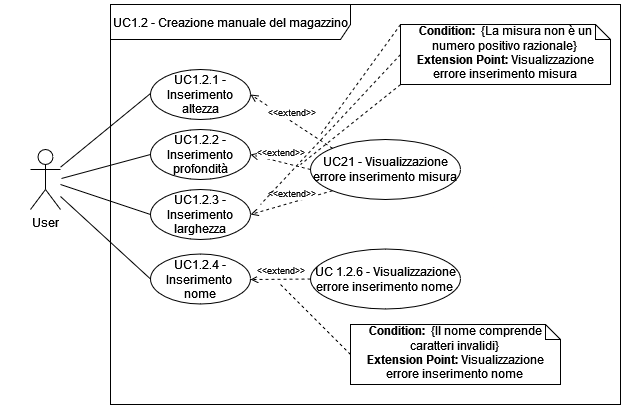
\includegraphics[width=0.8\textwidth]{UC_diagrams_1-10/UC1.2.drawio.png}
    \caption{Diagramma UML UC1.2 - Creazione manuale del magazzino}
\end{figure}
\begin{itemize}
    \item \textbf{Attori:} User.
    \item \textbf{Pre-condizione:} L'applicazione è avviata e funzionante e l'utente desidera creare un nuovo magazzino 3D.
    \item \textbf{Post-condizione:} Un nuovo magazzino vuoto viene creato e potrà essere visualizzato.
    \item \textbf{Scenario Principale:}  L’utente accede al sistema e sceglie la modalità di costruzione manuale. Inserisce i dati del magazzino, quali la planimetria [UC1.2.1], l'altezza [UC1.2.3] e il nome  [UC1.2.4], che vengono correttamente processati e il magazzino viene costruito.
    \item \textbf{Generalizzazioni:} -
    \item \textbf{Estensioni:} -
\end{itemize}


\paragraph{UC1.2.1 - Creazione planimetria personalizzata}
\begin{itemize}
    \item \textbf{Attori:} User.
    \item \textbf{Pre-condizione:}  L'applicazione è avviata e funzionante e l'utente ha scelto di creare manualmente un nuovo magazzino 3D.
    \item \textbf{Post-condizione:} Viene inserita la planimetria per il nuovo magazzino.
    \item \textbf{Scenario Principale:}  L’utente sceglie la forma e le relative misure da dare allo spazio del magazzino.
    \item \textbf{Generalizzazioni:} -
    \item \textbf{Estensioni:} È presente una estensione:
    \begin{itemize}
        \item UC1.2.2 - Visualizzazione errore creazione planimetria.
    \end{itemize}
\end{itemize}


\paragraph{UC1.2.2 - Visualizzazione errore creazione planimetria}
\begin{itemize}
    \item \textbf{Attori:} User.
    \item \textbf{Pre-condizione:}  L'utente ha inserito una planimetria invalida.
    \item \textbf{Post-condizione:} L'utente visualizza un messaggio d'errore e l'operazione fallisce.
    \item \textbf{Scenario Principale:} L'utente visualizza un messaggio informativo sull'errore e ne conferma la ricezione. L'operazione, di conseguenza, fallisce.
    \item \textbf{Generalizzazioni:} -
    \item \textbf{Estensioni:} -
\end{itemize}


\paragraph{UC1.2.3 - Inserimento altezza}
\begin{itemize}
    \item \textbf{Attori:} User.
    \item \textbf{Pre-condizione:}  L'applicazione è avviata e funzionante e l'utente ha scelto di creare manualmente un nuovo magazzino 3D.
    \item \textbf{Post-condizione:} Viene inserita l'altezza per il nuovo magazzino.
    \item \textbf{Scenario Principale:}  L’utente inserisce l'altezza del magazzino da costruire.
    \item \textbf{Generalizzazioni:} -
    \item \textbf{Estensioni:} È presente una estensione:
    \begin{itemize}
        \item UC21 - Visualizzazione errore inserimento misura.
    \end{itemize}
\end{itemize}


\paragraph{UC1.2.4 - Inserimento nome}
\begin{itemize}
    \item \textbf{Attori:} User.
    \item \textbf{Pre-condizione:}  L'applicazione è avviata e funzionante e l'utente ha scelto di creare manualmente un nuovo magazzino 3D.
    \item \textbf{Post-condizione:} Viene inserito il nome del nuovo magazzino.
    \item \textbf{Scenario Principale:}  L’utente inserisce il nome del magazzino da costruire.
    \item \textbf{Generalizzazioni:} -
    \item \textbf{Estensioni:} È presente una estensione:
    \begin{itemize}
        \item UC1.2.6 - Visualizzazione errore inserimento nome.
    \end{itemize}
\end{itemize}


\paragraph{UC1.2.5 - Visualizzazione errore inserimento nome}
\begin{itemize}
    \item \textbf{Attori:} User.
    \item \textbf{Pre-condizione:}  L'utente ha inserito come nome del magazzino un valore comprendente caratteri invalidi.
    \item \textbf{Post-condizione:} L'utente visualizza un messaggio d'errore e l'operazione fallisce.
    \item \textbf{Scenario Principale:}  L'utente visualizza un messaggio informativo sull'errore e ne conferma la ricezione. L'operazione, di conseguenza, fallisce.
    \item \textbf{Generalizzazioni:} -
    \item \textbf{Estensioni:} -
\end{itemize}


\subsubsection{UC1.3 - Visualizzazione errore caricamento file}
\begin{itemize}
    \item \textbf{Attori:} User.
    \item \textbf{Pre-condizione:} L'utente fornisce un file in un formato non supportato o con dati non validi.
    \item \textbf{Post-condizione:} L'utente visualizza un messaggio d'errore e l'operazione fallisce.
    \item \textbf{Scenario Principale:}  L'utente visualizza un messaggio informativo sull'errore e ne conferma la ricezione. L'operazione, di conseguenza, fallisce.
    \item \textbf{Generalizzazioni:} -
    \item \textbf{Estensioni:} -
\end{itemize}
\subsection{UC2 - Salvataggio magazzino}
\begin{figure}[H]
  \centering
  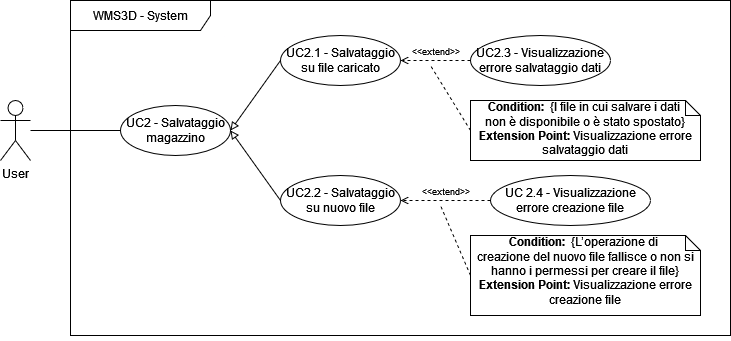
\includegraphics[width=0.8\textwidth]{UC_diagrams_1-10/UC2_sys.drawio.png}
   \caption{Diagramma UML UC2}
\end{figure}
\begin{itemize}
    \item \textbf{Attori:} User.
    \item \textbf{Pre-condizione:}  L'utente ha creato un magazzino [UC1] e lo sta visualizzando [UC3].
    \item \textbf{Post-condizione:} L'utente salva su un file locale i dati aggiornati di costruzione del magazzino.
    \item \textbf{Scenario Principale:}  L'utente decide di salvare la planimetria 3D del magazzino e sceglie una modalità di salvataggio o su file già caricato al momento della creazione [UC2.1] o su un nuovo file [UC2.2]. I dati vengono poi salvati correttamente dall'utente nel file specificato.
    \item \textbf{Generalizzazioni:} Sono presenti due generalizzazioni:
    \begin{itemize}
        \item UC2.1 - Salvataggio su file caricato;
        \item UC2.2 - Salvataggio su nuovo file.
    \end{itemize}
    \item \textbf{Estensioni:} -
\end{itemize}


\subsubsection{UC2.1 - Salvataggio su file caricato}
\begin{itemize}
    \item \textbf{Attori:} User.
    \item \textbf{Pre-condizione:} L'utente ha creato un magazzino attraverso caricamento da file [UC1.1] e lo sta visualizzando [UC3].
    \item \textbf{Post-condizione:} L'utente salva sul file locale caricato in precedenza i dati aggiornati di costruzione del magazzino.
    \item \textbf{Scenario Principale:} L'utente decide di salvare la planimetria 3D su file già caricato al momento della creazione [UC1.1]. I dati vengono poi salvati correttamente dall'utente nel file specificato.
    \item \textbf{Generalizzazioni:} -
    \item \textbf{Estensioni:} È presente una estensione:
    \begin{itemize}
        \item UC2.3 - Visualizzazione errore salvataggio dati.
    \end{itemize}
\end{itemize}


\subsubsection{UC2.2 - Salvataggio su nuovo file}
\begin{figure}[H]
  \centering
  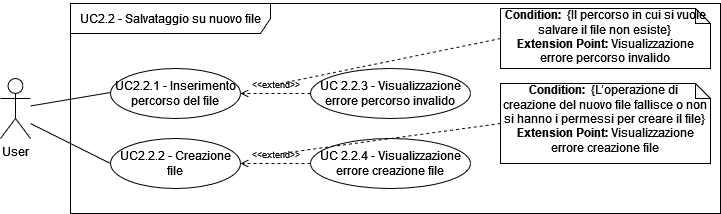
\includegraphics[width=0.8\textwidth]{UC_diagrams_1-10/UC2.2.drawio.png}
   \caption{Diagramma UML UC2.2}
\end{figure}
\begin{itemize}
    \item \textbf{Attori:} User.
    \item \textbf{Pre-condizione:} L'utente ha creato un magazzino [UC1] e lo sta visualizzando [UC3].
    \item \textbf{Post-condizione:} L'utente crea un nuovo file con i dati di costruzione del magazzino.
    \item \textbf{Scenario Principale:} L'utente decide di salvare la planimetria 3D su un nuovo file. Quindi decide in che cartella locale creare il nuovo file [UC2.2.1] e poi lo crea al suo interno [UC2.2.2].
    \item \textbf{Generalizzazioni:} -
    \item \textbf{Estensioni:} -
\end{itemize}


\paragraph{UC2.2.1 - Inserimento percorso del file}
\begin{itemize}
    \item \textbf{Attori:} User.
    \item \textbf{Pre-condizione:} L'utente vuole salvare i dati di costruzione del magazzino in un nuovo file.
    \item \textbf{Post-condizione:} L'utente inserisce il percorso in cui creare il nuovo file.
    \item \textbf{Scenario Principale:} L'utente decide di salvare la planimetria 3D su un nuovo file. Quindi decide in che cartella locale creare il nuovo file e la inserisce.
    \item \textbf{Generalizzazioni:} -
    \item \textbf{Estensioni:} È presente una estensione:
    \begin{itemize}
        \item UC2.2.3 - Visualizzazione errore percorso invalido.
    \end{itemize}
\end{itemize}


\paragraph{UC2.2.2 - Creazione file}
\begin{itemize}
    \item \textbf{Attori:} User.
    \item \textbf{Pre-condizione:}  L'utente vuole salvare i dati di costruzione del magazzino in un nuovo file e ha inserito il percorso in cui salvare questo nuovo file [UC2.2.1].
    \item \textbf{Post-condizione:} L'utente crea un nuovo file con i dati di costruzione del magazzino nella cartella specificata attraverso [UC2.2.1].
    \item \textbf{Scenario Principale:} L'utente decide di salvare la planimetria 3D su un nuovo file. Quindi crea il file, completo di tutti i dati, all'interno di una cartella specificata attraverso [UC2.2.1].
    \item \textbf{Generalizzazioni:} -
    \item \textbf{Estensioni:} È presente una estensione:
    \begin{itemize}
        \item UC2.2.4 - Visualizzazione errore creazione file.
    \end{itemize}    
\end{itemize}


\paragraph{UC2.2.3 - Visualizzazione errore percorso invalido}
\begin{itemize}
    \item \textbf{Attori:} User.
    \item \textbf{Pre-condizione:} Il percorso in cui l'utente vuole salvare il file non esiste.
    \item \textbf{Post-condizione:} L'utente visualizza un messaggio d'errore e il salvataggio fallisce.
    \item \textbf{Scenario Principale:} L'utente visualizza un messaggio informativo sull'errore e ne conferma la ricezione. L'operazione, di conseguenza, fallisce.
    \item \textbf{Generalizzazioni:} -
    \item \textbf{Estensioni:} -
\end{itemize}


\paragraph{UC2.2.4 - Visualizzazione errore creazione file}
\begin{itemize}
    \item \textbf{Attori:} User.
    \item \textbf{Pre-condizione:} L'operazione di creazione del nuovo file fallisce oppure non si hanno i permessi per creare il file.
    \item \textbf{Post-condizione:} L'utente visualizza un messaggio d'errore e il salvataggio fallisce.
    \item \textbf{Scenario Principale:} L'utente visualizza un messaggio informativo sull'errore e ne conferma la ricezione. L'operazione, di conseguenza, fallisce.
    \item \textbf{Generalizzazioni:} -
    \item \textbf{Estensioni:} -
\end{itemize}


\subsubsection{UC2.3 - Visualizzazione errore salvataggio dati}
\begin{itemize}
    \item \textbf{Attori:} User.
    \item \textbf{Pre-condizione:}  Il file in cui salvare i dati non è disponibile o è stato spostato. 
    \item \textbf{Post-condizione:} L'utente visualizza un messaggio d'errore e il salvataggio fallisce.
    \item \textbf{Scenario Principale:}  L'utente visualizza un messaggio informativo sull'errore e ne conferma la ricezione. L'operazione, di conseguenza, fallisce.
    \item \textbf{Generalizzazioni:} -
    \item \textbf{Estensioni:} -
\end{itemize}
\subsection{UC3 - Visualizzazione 3D del magazzino}
\begin{figure}[H]
  \centering
  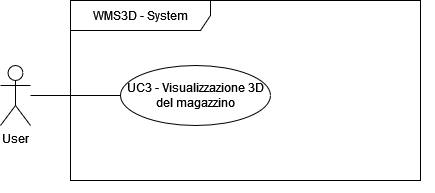
\includegraphics[width=0.8\textwidth]{UC_diagrams_1-10/UC3_sys.drawio.png}
   \caption{Diagramma UML UC3 - Visualizzazione 3D del magazzino}
\end{figure}
\begin{figure}[H]
  \centering
  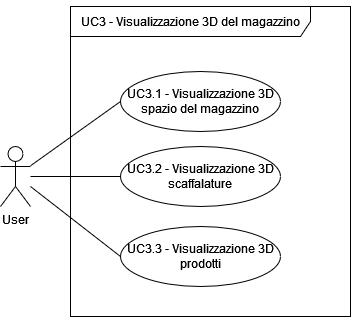
\includegraphics[width=0.5\textwidth]{UC_diagrams_1-10/UC3.drawio.png}
   \caption{Diagramma UML in dettaglio UC3 - Visualizzazione 3D del magazzino}
\end{figure}
\begin{itemize}
    \item \textbf{Attori:} User.
    \item \textbf{Pre-condizione:}  L'utente ha creato un magazzino [UC1].
    \item \textbf{Post-condizione:} L'utente può vedere il magazzino creato in 3D in tutte le sue parti.
    \item \textbf{Scenario Principale:}  L'utente visualizza interamente in 3D la planimetria del magazzino, in particolare può vedere lo spazio in sè del magazzino [UC3.1] e, se presenti, può visualizzare anche scaffalature [UC3.2] e prodotti [UC3.3].
    \item \textbf{Generalizzazioni:} -
    \item \textbf{Estensioni:} -
\end{itemize}


\subsubsection{UC3.1 - Visualizzazione 3D spazio del magazzino}
\begin{figure}[H]
  \centering
  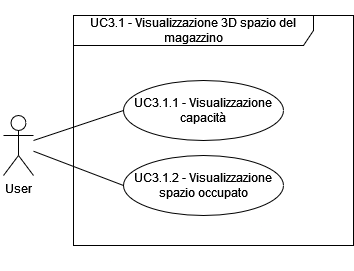
\includegraphics[width=0.6\textwidth]{UC_diagrams_1-10/UC3.1.drawio.png}
   \caption{Diagramma UML UC3.1 - Visualizzazione 3D spazio del magazzino}
\end{figure}
\begin{itemize}
    \item \textbf{Attori:} User.
    \item \textbf{Pre-condizione:} L'utente ha creato un magazzino [UC1].
    \item \textbf{Post-condizione:} L'utente visualizza in 3D lo spazio del magazzino.
    \item \textbf{Scenario Principale:}  L'utente può vederne in 3D lo spazio del magazzino, in particolare può notarne graficamente e in proporzione capacità del magazzino [UC3.1.1] e spazio occupato al suo interno [UC3.1.2].
    \item \textbf{Generalizzazioni:} -
    \item \textbf{Estensioni:} -
\end{itemize}


\paragraph{UC3.1.1 - Visualizzazione capacità}
\begin{itemize}
    \item \textbf{Attori:} User.
    \item \textbf{Pre-condizione:} L'utente ha creato un magazzino [UC1] e ne sta guardando lo spazio.
    \item \textbf{Post-condizione:} L'utente visualizza la capacità del magazzino.
    \item \textbf{Scenario Principale:}  L'utente, guardando allo spazio del magazzino creato dal render 3D, può notare la capacità (i.e. la grandezza) del magazzino.
    \item \textbf{Generalizzazioni:} -
    \item \textbf{Estensioni:} -
\end{itemize}


\paragraph{UC3.1.2 - Visualizzazione spazio occupato}
\begin{itemize}
    \item \textbf{Attori:} User.
    \item \textbf{Pre-condizione:} L'utente ha creato un magazzino [UC1] e ne sta guardando lo spazio.
    \item \textbf{Post-condizione:} L'utente visualizza lo spazio occupato all'interno del magazzino.
    \item \textbf{Scenario Principale:}  L'utente, guardando allo spazio del magazzino creato dal render 3D, può notare lo spazio occupato (i.e. la proporzione tra parti in cui sono posizionate scaffalature e parti vuote).
    \item \textbf{Generalizzazioni:} -
    \item \textbf{Estensioni:} -
\end{itemize}


\subsubsection{UC3.2 - Visualizzazione 3D scaffalature}
\begin{figure}[H]
  \centering
  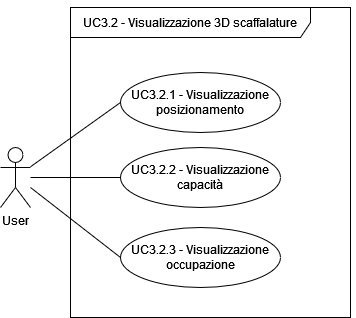
\includegraphics[width=0.6\textwidth]{UC_diagrams_1-10/UC3.2.drawio.png}
   \caption{Diagramma UML UC3.2 - Visualizzazione 3D scaffalature}
\end{figure}
\begin{itemize}
    \item \textbf{Attori:} User.
    \item \textbf{Pre-condizione:} L'utente ha creato un magazzino [UC1] al cui interno sono presenti delle scaffalature.
    \item \textbf{Post-condizione:} L'utente visualizza in 3D le scaffalature all'interno del magazzino.
    \item \textbf{Scenario Principale:}  L'utente può vedere in 3D le scaffalature all'interno del magazzino, in particolare potrà notarne (graficamente) il posizionamento [UC3.2.1], la capacità [UC3.2.2] e lo spazio occupato al suo interno [UC3.2.3].
    \item \textbf{Generalizzazioni:} -
    \item \textbf{Estensioni:} -
\end{itemize}


\paragraph{UC3.2.1 - Visualizzazione posizionamento}
\begin{itemize}
    \item \textbf{Attori:} User.
    \item \textbf{Pre-condizione:} L'utente ha creato un magazzino [UC1] al cui interno sono presenti delle scaffalature a cui l'utente sta guardando.
    \item \textbf{Post-condizione:} L'utente visualizza il posizionamento delle scaffalature all'interno del magazzino.
    \item \textbf{Scenario Principale:} L'utente, guardando alle scaffalature presenti nel magazzino dal render 3D, può notarne la loro posizione e disposizione all'interno del magazzino.
    \item \textbf{Generalizzazioni:} -
    \item \textbf{Estensioni:} -
\end{itemize}


\paragraph{UC3.2.2 - Visualizzazione capacità}
\begin{itemize}
    \item \textbf{Attori:} User.
    \item \textbf{Pre-condizione:} L'utente ha creato un magazzino [UC1] al cui interno sono presenti delle scaffalature a cui l'utente sta guardando.
    \item \textbf{Post-condizione:} L'utente visualizza la capacità delle scaffalature all'interno dell magazzino.
    \item \textbf{Scenario Principale:}  L'utente, guardando alle scaffalature presenti nel magazzino dal render 3D, può notarne la loro capacità, ovvero il numero di bin\textsuperscript{G} da cui sono composte.
    \item \textbf{Generalizzazioni:} -
    \item \textbf{Estensioni:} -
\end{itemize}


\paragraph{UC3.2.3 - Visualizzazione occupazione}
\begin{itemize}
    \item \textbf{Attori:} User.
    \item \textbf{Pre-condizione:} L'utente ha creato un magazzino [UC1] al cui interno sono presenti delle scaffalature a cui l'utente sta guardando.
    \item \textbf{Post-condizione:} L'utente visualizza lo stato di occupazione delle scaffalature all'interno del magazzino.
    \item \textbf{Scenario Principale:}  L'utente, guardando alle scaffalature presenti nel magazzino dal render 3D, può notarne la loro occupazione (i.e. la proporzione tra parti in cui sono posizionati prodotti e le parti libere).
    \item \textbf{Generalizzazioni:} -
    \item \textbf{Estensioni:} -
\end{itemize}


\subsubsection{UC3.3 - Visualizzazione 3D prodotti}
\begin{figure}[H]
  \centering
  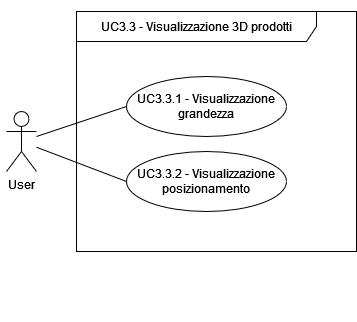
\includegraphics[width=0.6\textwidth]{UC_diagrams_1-10/UC3.3.drawio.png}
   \caption{Diagramma UML UC3.3 - Visualizzazione 3D prodotti}
\end{figure}
\begin{itemize}
    \item \textbf{Attori:} User.
    \item \textbf{Pre-condizione:}  L'utente ha creato un magazzino [UC1] al cui interno sono presenti delle scaffalature e dei prodotti posizionati.
    \item \textbf{Post-condizione:} L'utente visualizza in 3D i prodotti posizionati nelle scaffalature all'interno del magazzino.
    \item \textbf{Scenario Principale:}  L'utente può vedere in 3D i prodotti posizionati sulle scaffalature all'interno del magazzino, in particolare potrà notarne (graficamente) la grandezza [UC3.3.1] e il posizionamento [UC3.3.2].
    \item \textbf{Generalizzazioni:} -
    \item \textbf{Estensioni:} -
\end{itemize}


\paragraph{UC3.3.1 - Visualizzazione grandezza}
\begin{itemize}
    \item \textbf{Attori:} User.
    \item \textbf{Pre-condizione:} L'utente ha creato un magazzino [UC1] al cui interno sono presenti delle scaffalature e dei prodotti posizionati. L'utente sua guardando questi ultimi.
    \item \textbf{Post-condizione:} L'utente visualizza la grandezza dei prodotti posizionati nelle scaffalature all'interno del magazzino.
    \item \textbf{Scenario Principale:} L'utente, guardando ai prodotti presenti nel magazzino dal render 3D, può notarne la loro dimensione.
    \item \textbf{Generalizzazioni:} -
    \item \textbf{Estensioni:} -
\end{itemize}


\paragraph{UC3.3.2 - Visualizzazione posizionamento}
\begin{itemize}
    \item \textbf{Attori:} User.
    \item \textbf{Pre-condizione:} L'utente ha creato un magazzino [UC1] al cui interno sono presenti delle scaffalature e dei prodotti posizionati. L'utente sua guardando questi ultimi.
    \item \textbf{Post-condizione:} L'utente visualizza in quali scaffalature sono posizionati i prodotti all'interno del magazzino.
    \item \textbf{Scenario Principale:}  L'utente, guardando ai prodotti presenti nel magazzino dal render 3D, può notarne il loro posizionamento e disposizione (i.e. in quale scaffalatura e in quale bin i prodotti sono posizionati).
    \item \textbf{Generalizzazioni:} -
    \item \textbf{Estensioni:} -
\end{itemize}
\subsection{UC4 - Visualizzazione libreria}
\begin{figure}[H]
  \centering
  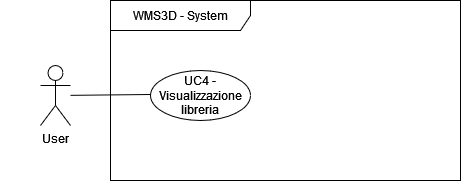
\includegraphics[width=0.8\textwidth]{UC_diagrams_1-10/UC4_sys.drawio.png}
   \caption{Diagramma UML UC4 - Visualizzazione libreria}
\end{figure}
\begin{figure}[H]
  \centering
  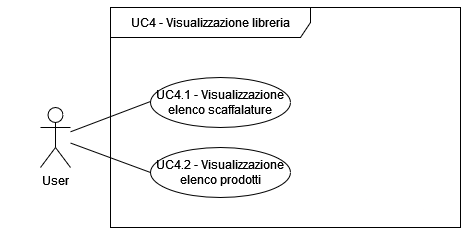
\includegraphics[width=0.8\textwidth]{UC_diagrams_1-10/UC4.drawio.png}
   \caption{Diagramma UML in dettaglio UC4 - Visualizzazione libreria}
\end{figure}
\begin{itemize}
    \item \textbf{Attori:} User.
    \item \textbf{Pre-condizione:}  L'utente ha creato un magazzino [UC1].
    \item \textbf{Post-condizione:} L'utente visualizza in una parte dell'applicazione uno spazio riservato alle informazioni testuali riguardanti gli elementi (scaffalature e prodotti) interni al magazzino (i.e. la libreria\textsuperscript{G}).
    \item \textbf{Scenario Principale:}  L'utente può visualizzare in libreria, un elenco delle scaffalature [UC4.1] e uno dei prodotti [UC4.2] (con relativi dati), sempre se presenti all'interno del magazzino. Se non vi dovessero essere nessuno di questi elementi, lo spazio verrà visualizzato vuoto.
    \item \textbf{Generalizzazioni:} -
    \item \textbf{Estensioni:} -
\end{itemize}


\subsubsection{UC4.1 - Visualizzazione elenco scaffalature}
\begin{figure}[H]
  \centering
  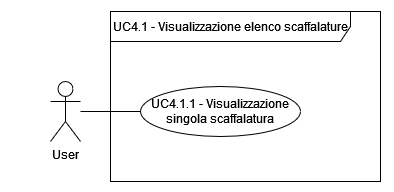
\includegraphics[width=0.8\textwidth]{UC_diagrams_1-10/UC4.1.drawio.png}
   \caption{Diagramma UML UC4.1 - Visualizzazione elenco scaffalature}
\end{figure}
\begin{itemize}
    \item \textbf{Attori:} User.
    \item \textbf{Pre-condizione:}  L'utente ha creato un magazzino [UC1] e ne sta guardando la libreria.
    \item \textbf{Post-condizione:} L'utente può vedere i dati relativi a tutte le scaffalature presenti nel magazzino.
    \item \textbf{Scenario Principale:} L'utente può visualizzare in libreria ogni singola scaffalatura [UC4.1.1] (con relativi dati), sempre se presenti all'interno del magazzino. Se non vi dovesse essere nessuna scaffalatura, l'elenco sarà nullo.
    \item \textbf{Generalizzazioni:} -
    \item \textbf{Estensioni:} -
\end{itemize}


\paragraph{UC4.1.1 - Visualizzazione singola scaffalatura}
\begin{figure}[H]
  \centering
  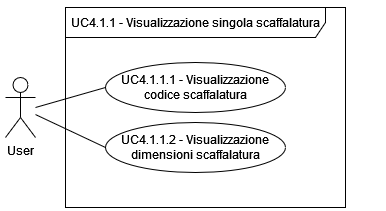
\includegraphics[width=0.7\textwidth]{UC_diagrams_1-10/UC4.1.1.drawio.png}
   \caption{Diagramma UML UC4.1.1 - Visualizzazione singola scaffalatura}
\end{figure}
\begin{itemize}
    \item \textbf{Attori:} User.
    \item \textbf{Pre-condizione:} L'utente ha creato un magazzino [UC1] e sta guardando all'elenco delle scaffalature interno alla libreria. Almeno una scaffalatura deve essere creata [UC6] e posizionata [UC7].
    \item \textbf{Post-condizione:} L'utente può vedere i dati relativi ad una singola scaffalatura.
    \item \textbf{Scenario Principale:} L'utente può visualizzare il codice identificativo [UC4.1.1.1] e le dimensioni [UC4.1.1.2] per ogni singola scaffalatura presente nella libreria.
    \item \textbf{Generalizzazioni:} -
    \item \textbf{Estensioni:} -
\end{itemize}


\paragraph{UC4.1.1.1 - Visualizzazione codice scaffalatura}
\begin{itemize}
    \item \textbf{Attori:} User.
    \item \textbf{Pre-condizione:} L'utente ha creato un magazzino [UC1] e sta guardando ad una singola scaffalatura all'interno della libreria. Pertanto, almeno una scaffalatura deve essere creata [UC6] e posizionata [UC7].
    \item \textbf{Post-condizione:} L'utente può vedere il codice relativo alla singola scaffalatura.
    \item \textbf{Scenario Principale:} L'utente può visualizzare il codice identificativo per ogni singola scaffalatura presente nella libreria.
    \item \textbf{Generalizzazioni:} -
    \item \textbf{Estensioni:} -
\end{itemize}


\paragraph{UC4.1.1.2 - Visualizzazione dimensioni scaffalatura}
\begin{figure}[H]
  \centering
  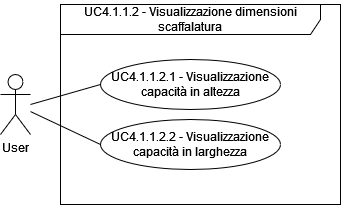
\includegraphics[width=0.8\textwidth]{UC_diagrams_1-10/UC4.1.1.2.drawio.png}
   \caption{Diagramma UML UC4.1.1.2 - Visualizzazione dimensioni scaffalatura}
\end{figure}
\begin{itemize}
    \item \textbf{Attori:} User.
    \item \textbf{Pre-condizione:} L'utente ha creato un magazzino [UC1] e sta guardando ad una singola scaffalatura all'interno della libreria. Pertanto, almeno una scaffalatura deve essere creata [UC6] e posizionata [UC7].
    \item \textbf{Post-condizione:} L'utente può vedere le dimensioni relative alla singola scaffalatura.
    \item \textbf{Scenario Principale:} L'utente può visualizzare le dimensioni, quindi capacità in altezza [UC4.1.1.2.1] e capacità in larghezza [UC4.1.1.2.2], per ogni singola scaffalatura presente nella libreria.
    \item \textbf{Generalizzazioni:} -
    \item \textbf{Estensioni:} -
\end{itemize}


\paragraph{UC4.1.1.2.1 - Visualizzazione capacità in altezza}
\begin{itemize}
    \item \textbf{Attori:} User.
    \item \textbf{Pre-condizione:} L'utente ha creato un magazzino [UC1] e sta guardando ad una singola scaffalatura all'interno della libreria. Pertanto, almeno una scaffalatura deve essere creata [UC6] e posizionata [UC7].
    \item \textbf{Post-condizione:} L'utente può vedere la capacità in altezza relativa alla singola scaffalatura.
    \item \textbf{Scenario Principale:} L'utente può visualizzare la capacità (i.e. numero di bin) in altezza per ogni singola scaffalatura presente nella libreria.
    \item \textbf{Generalizzazioni:} -
    \item \textbf{Estensioni:} -
\end{itemize}


\paragraph{UC4.1.1.2.2 - Visualizzazione capacità in larghezza}
\begin{itemize}
    \item \textbf{Attori:} User.
    \item \textbf{Pre-condizione:} L'utente ha creato un magazzino [UC1] e sta guardando ad una singola scaffalatura all'interno della libreria. Pertanto, almeno una scaffalatura deve essere creata [UC6] e posizionata [UC7].
    \item \textbf{Post-condizione:} L'utente può vedere la capacità in larghezza relativa alla singola scaffalatura.
    \item \textbf{Scenario Principale:}  L'utente può visualizzare la capacità (i.e. numero di bin) in larghezza per ogni singola scaffalatura presente nella libreria.
    \item \textbf{Generalizzazioni:} -
    \item \textbf{Estensioni:} -
\end{itemize}


\subsubsection{UC4.2 - Visualizzazione elenco prodotti}
\begin{figure}[H]
  \centering
  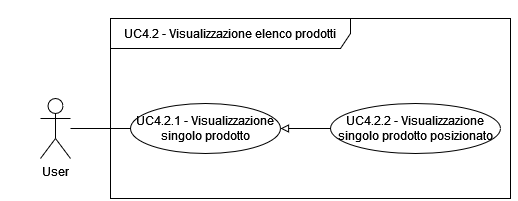
\includegraphics[width=0.8\textwidth]{UC_diagrams_1-10/UC4.2.drawio.png}
   \caption{Diagramma UML UC4.2 - Visualizzazione elenco prodotti}
\end{figure}
\begin{itemize}
    \item \textbf{Attori:} User.
    \item \textbf{Pre-condizione:}  L'utente ha creato un magazzino [UC1] e ne sta guardando la libreria.
    \item \textbf{Post-condizione:} L'utente può vedere i dati relativi a tutti i prodotti presenti nel magazzino.
    \item \textbf{Scenario Principale:} L'utente può visualizzare in libreria ogni singolo prodotto [UC4.2.1] (con relativi dati), posizionato o meno. Se non vi dovesse essere nessun prodotto, l'elenco sarà nullo.
    \item \textbf{Generalizzazioni:} -
    \item \textbf{Estensioni:} -
\end{itemize}


\paragraph{UC4.2.1 - Visualizzazione singolo prodotto}
\begin{figure}[H]
  \centering
  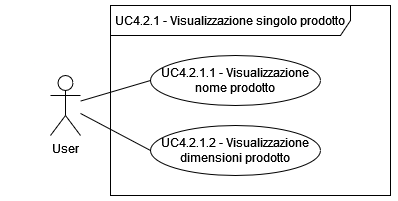
\includegraphics[width=0.8\textwidth]{UC_diagrams_1-10/UC4.2.1.drawio.png}
   \caption{Diagramma UML UC4.2.1 - Visualizzazione singolo prodotto}
\end{figure}
\begin{itemize} 
    \item \textbf{Attori:} User.
    \item \textbf{Pre-condizione:}  L'utente ha creato un magazzino [UC1] e sta guardando all'elenco dei prodotti interno alla libreria. Almeno un prodotto deve essere stato creato [UC13].
    \item \textbf{Post-condizione:} L'utente può vedere i dati relativi ad un singolo prodotto.
    \item \textbf{Scenario Principale:} L'utente può visualizzare il nome [UC4.2.1.1] per ogni singolo prodotto presente nella libreria. 
    \item \textbf{Generalizzazioni:} È presente una generalizzazione:
    \begin{itemize}
        \item UC4.2.2 - Visualizzazione singolo prodotto posizionato
    \end{itemize}
    \item \textbf{Estensioni:} -
\end{itemize}


\paragraph{UC4.2.1.1 - Visualizzazione nome prodotto}
\begin{itemize} 
    \item \textbf{Attori:} User.
    \item \textbf{Pre-condizione:}  L'utente ha creato un magazzino [UC1] e sta guardando ad un singolo prodotto all'interno della libreria. Almeno un prodotto deve essere stato creato [UC13].
    \item \textbf{Post-condizione:} L'utente può vedere il nome del prodotto.
    \item \textbf{Scenario Principale:} L'utente può visualizzare il nome per ogni singolo prodotto presente nella libreria. 
    \item \textbf{Generalizzazioni:} -
    \item \textbf{Estensioni:} -
\end{itemize}


\paragraph{UC4.2.2 - Visualizzazione singolo prodotto posizionato}
\begin{figure}[H]
  \centering
  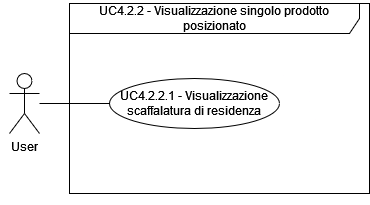
\includegraphics[width=0.8\textwidth]{UC_diagrams_1-10/UC4.2.2.drawio.png}
   \caption{Diagramma UML UC4.2.2 - Visualizzazione singolo prodotto posizionato}
\end{figure}
\begin{itemize}
    \item \textbf{Attori:} User.
    \item \textbf{Pre-condizione:}  L'utente ha creato un magazzino [UC1] e sta guardando all'elenco dei prodotti interno alla libreria. Almeno un prodotto deve essere stato creato [UC13] e posizionato [UC14].
    \item \textbf{Post-condizione:}  L'utente può vedere i dati relativi ad un singolo prodotto.
    \item \textbf{Scenario Principale:}  L'utente può visualizzare il nome [UC4.2.1.1] e le dimensioni [UC4.2.1.2] per ogni singolo prodotto ed, essendo posizionato, anche la scaffalatura in cui il prodotto risiede [4.2.2.1]. 
    \item \textbf{Generalizzazioni:} -
    \item \textbf{Estensioni:} -
\end{itemize}


\paragraph{UC4.2.2.1 - Visualizzazione scaffalatura di residenza}
\begin{itemize} 
    \item \textbf{Attori:} User.
    \item \textbf{Pre-condizione:}  L'utente ha creato un magazzino [UC1] e sta guardando ad un singolo prodotto all'interno della libreria. Almeno un prodotto deve essere stato creato [UC13] e posizionato [UC14].
    \item \textbf{Post-condizione:} L'utente può vedere la scaffalatura di residenza di un prodotto posizionato.
    \item \textbf{Scenario Principale:} L'utente può visualizzare la posizione, ovvero il codice della scaffalatura in cui il prodotto si trova, per ogni singolo prodotto posizionato presente nella libreria. 
    \item \textbf{Generalizzazioni:} -
    \item \textbf{Estensioni:} -
\end{itemize}
\subsection{UC5 - Modifica vista magazzino}
\begin{figure}[H]
  \centering
  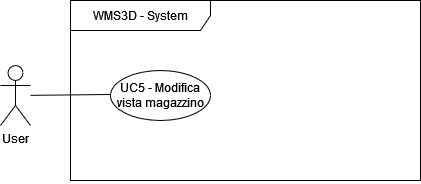
\includegraphics[width=0.8\textwidth]{UC_diagrams_1-10/UC5_sys.drawio.png}
   \caption{Diagramma UML UC5}
\end{figure}
\begin{figure}[H]
  \centering
  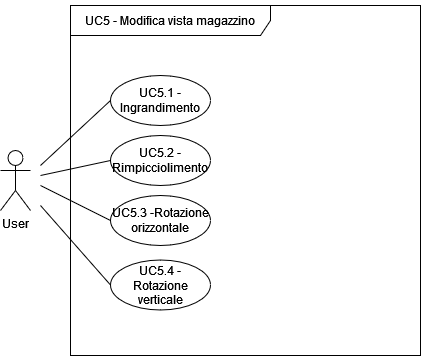
\includegraphics[width=0.8\textwidth]{UC_diagrams_1-10/UC5.drawio.png}
   \caption{Diagramma UML UC5 - dettaglio}
\end{figure}
\begin{itemize}
    \item \textbf{Attori:} User.
    \item \textbf{Pre-condizione:}  L'utente sta visualizzando il magazzino in 3D [UC3].
    \item \textbf{Post-condizione:} L'utente visualizza il magazzino dal render 3D in maniera diversa.
    \item \textbf{Scenario Principale:}  L'utente può modificare la vista del render 3D del magazzino. In particolare, può visualizzare il magazzino più da vicino [UC5.1] o più da lontano [UC5.2], oppure può vedere il magazzino da una diversa angolazione, sia traslata orizzontalmente [UC5.3] sia verticalmente [UC5.4].
    \item \textbf{Generalizzazioni:} -
    \item \textbf{Estensioni:} -
\end{itemize}


\subsubsection{UC5.1 - Ingrandimento}
\begin{itemize}
    \item \textbf{Attori:} User.
    \item \textbf{Pre-condizione:}  L'utente sta visualizzando il magazzino in 3D [UC3].
    \item \textbf{Post-condizione:} L'utente osserva il magazzino nel render 3D più da vicino.
    \item \textbf{Scenario Principale:}  L'utente può visualizzare il magazzino più da vicino rispetto alla visualizzazione precedente.
    \item \textbf{Generalizzazioni:} -
    \item \textbf{Estensioni:} -
\end{itemize}


\subsubsection{UC5.2 - Rimpicciolimento}
\begin{itemize}
    \item \textbf{Attori:} User.
    \item \textbf{Pre-condizione:}  L'utente sta visualizzando il magazzino in 3D [UC3].
    \item \textbf{Post-condizione:} L'utente osserva il magazzino nel render 3D più da lontano.
    \item \textbf{Scenario Principale:}  L'utente può visualizzare il magazzino più da lontano [UC5.2] rispetto alla visualizzazione precedente.
    \item \textbf{Generalizzazioni:} -
    \item \textbf{Estensioni:} -
\end{itemize}


\subsubsection{UC5.3 - Rotazione orizzontale}
\begin{itemize}
    \item \textbf{Attori:} User.
    \item \textbf{Pre-condizione:}  L'utente sta visualizzando il magazzino in 3D [UC3].
    \item \textbf{Post-condizione:} L'utente osserva il magazzino nel render 3D da un'angolazione diversa, traslata orizzontalmente.
    \item \textbf{Scenario Principale:}  L'utente può visualizzare il magazzino da una diversa angolazione, spostata orizzontalmente rispetto alla visualizzazione precedente.
    \item \textbf{Generalizzazioni:} -
    \item \textbf{Estensioni:} -
\end{itemize}


\subsubsection{UC5.4 - Rotazione verticale}
\begin{itemize}
    \item \textbf{Attori:} User.
    \item \textbf{Pre-condizione:}  L'utente sta visualizzando il magazzino in 3D [UC3].
    \item \textbf{Post-condizione:} L'utente osserva il magazzino nel render 3D da un'angolazione diversa, traslata verticalmente.
    \item \textbf{Scenario Principale:} L'utente può visualizzare il magazzino da una diversa angolazione, spostata verticalmente rispetto alla visualizzazione precedente.
    \item \textbf{Generalizzazioni:} -
    \item \textbf{Estensioni:} -
\end{itemize}
\subsection{UC6 - Creazione scaffalatura}
\begin{figure}[H]
  \centering
  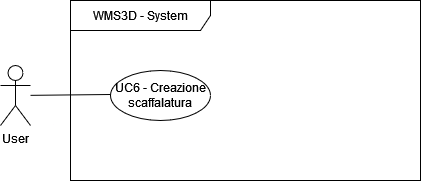
\includegraphics[width=0.8\textwidth]{UC_diagrams_1-10/UC6_sys.drawio.png}
   \caption{Diagramma UML UC6 - Creazione scaffalatura}
\end{figure}
\begin{figure}[H]
  \centering
  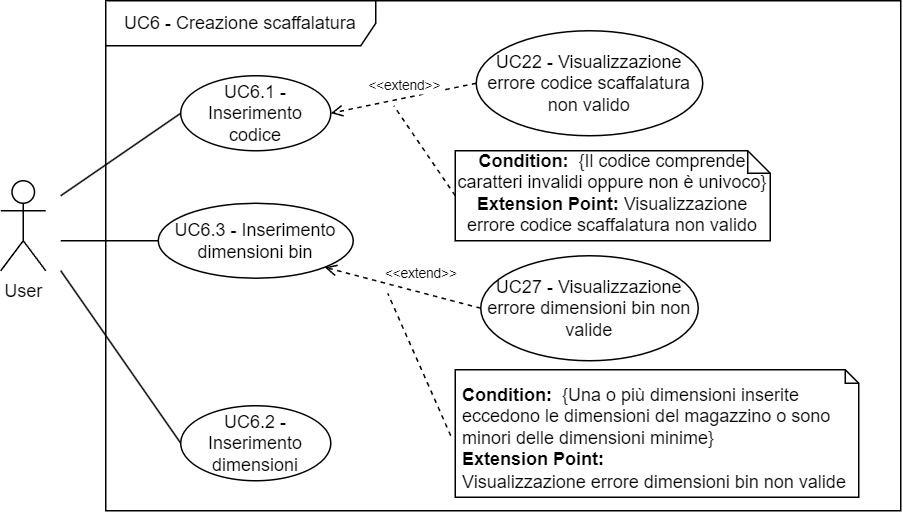
\includegraphics[width=0.8\textwidth]{UC_diagrams_1-10/UC6.drawio.png}
   \caption{Diagramma UML in dettaglio UC6 - Creazione scaffalatura}
\end{figure}
\begin{itemize}
    \item \textbf{Attori:} User.
    \item \textbf{Pre-condizione:}  L'utente ha creato/caricato un magazzino [UC1].
    \item \textbf{Post-condizione:} L'utente crea una scaffalatura, aggiunta in libreria, e che dovrà essere obbligatoriamente posizionata [UC7].
    \item \textbf{Scenario Principale:}  L'utente crea una scaffalatura, inserendo un codice univoco [UC6.1], le dimensioni del singolo bin della scaffalatura [UC6.3] e le dimensioni della scaffalatura in unità di bin [UC6.2].
    \item \textbf{Generalizzazioni:} -
    \item \textbf{Estensioni:} -
\end{itemize}


\subsubsection{UC6.1 - Inserimento codice}
\begin{itemize}
    \item \textbf{Attori:} User.
    \item \textbf{Pre-condizione:}  L'utente ha creato/caricato un magazzino [UC1] e vuole creare una nuova scaffalatura.
    \item \textbf{Post-condizione:} L'utente ha dato un codice identificativo per la nuova scaffalatura.
    \item \textbf{Scenario Principale:}  L'utente sceglie un codice univoco da dare alla scaffalatura.
    \item \textbf{Generalizzazioni:} 
    \item \textbf{Estensioni:} È presente una estensione nel caso in cui il codice non sia valido:
    \begin{itemize}
        \item UC22 - Visualizzazione errore codice scaffalatura non valido.
    \end{itemize}
\end{itemize}


\subsubsection{UC6.2 - Inserimento dimensioni}
\begin{figure}[H]
  \centering
  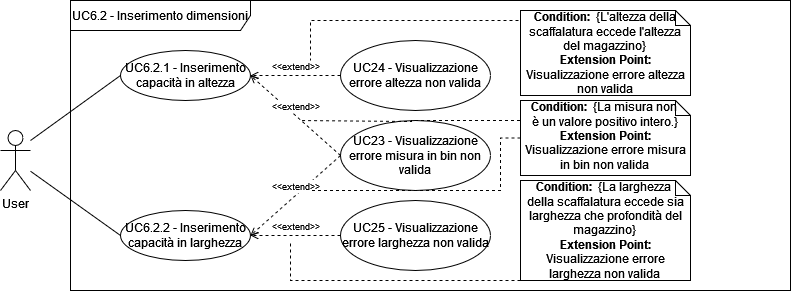
\includegraphics[width=0.9\textwidth]{UC_diagrams_1-10/UC6.2.drawio.png}
   \caption{Diagramma UML UC6.2 - Inserimento dimensioni}
\end{figure}
\begin{itemize}
    \item \textbf{Attori:} User.
    \item \textbf{Pre-condizione:} L'utente ha creato/caricato un magazzino [UC1] e vuole creare una nuova scaffalatura. L'utente deve aver inserito le dimensioni del singolo bin nella scaffalatura [UC6.3].
    \item \textbf{Post-condizione:}  L'utente ha inserito le dimensioni della nuova scaffalatura.
    \item \textbf{Scenario Principale:}  L'utente decide la capacità (numero di bin) in altezza e in larghezza da dare alla scaffalatura. Se le misure sono valide, la scaffalatura sarà creata.
    \item \textbf{Generalizzazioni:} -
    \item \textbf{Estensioni:} -
\end{itemize}


\paragraph{UC6.2.1 - Inserimento capacità in altezza}
\begin{itemize}
    \item \textbf{Attori:} User.
    \item \textbf{Pre-condizione:} L'utente ha creato/caricato un magazzino [UC1] e vuole creare una nuova scaffalatura. L'utente deve aver inserito le dimensioni del singolo bin nella scaffalatura [UC6.3].
    \item \textbf{Post-condizione:}  L'utente ha inserito la capacità in altezza della nuova scaffalatura.
    \item \textbf{Scenario Principale:}  L'utente decide il numero di bin in altezza da dare alla scaffalatura. 
    \item \textbf{Generalizzazioni:} -
    \item \textbf{Estensioni:} Sono presenti due estensioni:
    \begin{itemize}
        \item UC23 - Visualizzazione errore misura in bin non valida, nel caso in cui l'altezza non sia in un formato accettabile;
        \item UC24 - Visualizzazione errore altezza non valida, nel caso in cui l'altezza per la scaffalatura superi quella del magazzino.
    \end{itemize}
\end{itemize}


\paragraph{UC6.2.2 - Inserimento capacità in larghezza}
\begin{itemize}
    \item \textbf{Attori:} User.
    \item \textbf{Pre-condizione:} L'utente ha creato/caricato un magazzino [UC1] e vuole creare una nuova scaffalatura. L'utente deve aver inserito le dimensioni del singolo bin nella scaffalatura [UC6.3].
    \item \textbf{Post-condizione:}  L'utente ha inserito la capacità in larghezza della nuova scaffalatura.
    \item \textbf{Scenario Principale:}  L'utente decide il numero di bin in larghezza da dare alla scaffalatura.
    \item \textbf{Generalizzazioni:} -
    \item \textbf{Estensioni:}Sono presenti due estensioni:
    \begin{itemize}
        \item UC23 - Visualizzazione errore misura in bin non valida, nel caso in cui l'altezza non sia in un formato accettabile;
        \item UC25 - Visualizzazione errore larghezza non valida, nel caso in cui la larghezza per la scaffalatura superi quella del magazzino.
    \end{itemize}
\end{itemize}


\subsubsection{UC6.3 - Inserimento dimensioni bin}
\begin{figure}[H]
  \centering
  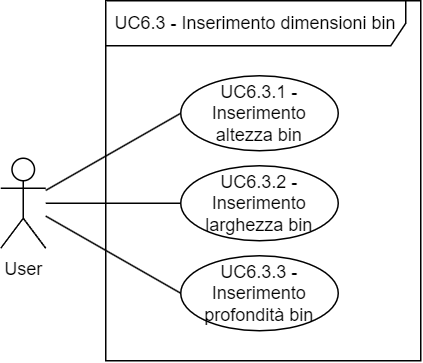
\includegraphics[width=0.5\textwidth]{UC_diagrams_1-10/UC6.3.drawio.png}
   \caption{Diagramma UML UC6.3 - Inserimento dimensioni bin}
\end{figure}
\begin{itemize}
    \item \textbf{Attori:} User.
    \item \textbf{Pre-condizione:} L'utente ha creato/caricato un magazzino [UC1] e vuole creare una nuova scaffalatura.
    \item \textbf{Post-condizione:}  L'utente ha inserito le dimensioni del singolo bin della nuova scaffalatura.
    \item \textbf{Scenario Principale:}  L'utente stabilisce la dimensione del singolo bin della scaffalatura, inserendo altezza, lunghezza e profondità.
    \item \textbf{Generalizzazioni:} -
    \item \textbf{Estensioni:} È presente una estensione nel caso in cui le dimensioni inserite eccedano la dimensione del magazzino oppure siano più piccole delle dimensioni minime previste:
    \begin{itemize}
        \item UC27 - Visualizzazione errore dimensioni bin non valide.
    \end{itemize}
\end{itemize}


\paragraph{UC6.3.1 - Inserimento altezza bin}
\begin{itemize}
    \item \textbf{Attori:} User.
    \item \textbf{Pre-condizione:} L'utente ha creato/caricato un magazzino [UC1] e vuole creare una nuova scaffalatura.
    \item \textbf{Post-condizione:}  L'utente ha inserito la dimensione dell'altezza per i bin della nuova scaffalatura.
    \item \textbf{Scenario Principale:}  L'utente decide la dimensione in altezza da dare ai bin della scaffalatura. 
    \item \textbf{Generalizzazioni:} -
    \item \textbf{Estensioni:} -
\end{itemize}


\paragraph{UC6.3.2 - Inserimento larghezza bin}
\begin{itemize}
    \item \textbf{Attori:} User.
    \item \textbf{Pre-condizione:} L'utente ha creato/caricato un magazzino [UC1] e vuole creare una nuova scaffalatura.
    \item \textbf{Post-condizione:}  L'utente ha inserito la dimensione della larghezza per i bin della nuova scaffalatura.
    \item \textbf{Scenario Principale:}  L'utente decide la dimensione in larghezza da dare ai bin della scaffalatura. 
    \item \textbf{Generalizzazioni:} -
    \item \textbf{Estensioni:} -
\end{itemize}


\paragraph{UC6.3.3 - Inserimento profondità bin}
\begin{itemize}
    \item \textbf{Attori:} User.
    \item \textbf{Pre-condizione:} L'utente ha creato/caricato un magazzino [UC1] e vuole creare una nuova scaffalatura.
    \item \textbf{Post-condizione:}  L'utente ha inserito la dimensione della profondità per i bin della nuova scaffalatura.
    \item \textbf{Scenario Principale:}  L'utente decide la dimensione in profondità da dare ai bin della scaffalatura. 
    \item \textbf{Generalizzazioni:} -
    \item \textbf{Estensioni:} -
\end{itemize}
\subsection{UC7 - Posizionamento scaffalatura}
\begin{figure}[H]
  \centering
  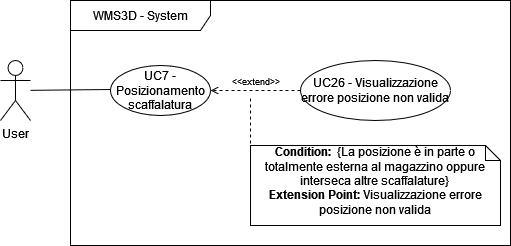
\includegraphics[width=0.8\textwidth]{UC_diagrams_1-10/UC7.drawio.png}
   \caption{Diagramma UML UC7 - Posizionamento scaffalatura}
\end{figure}
\begin{itemize}
    \item \textbf{Attori:} User.
    \item \textbf{Pre-condizione:}  L'utente ha creato una scaffalatura [UC6] e sta visualizzando il magazzino in 3D [UC3].
    \item \textbf{Post-condizione:} La scaffalatura creata è posizionata all'interno del render 3D.
    \item \textbf{Scenario Principale:} L'utente dopo aver creato una scaffalatura sceglie dove e come posizionarla all'interno del magazzino.
    \item \textbf{Generalizzazioni:} -
    \item \textbf{Estensioni:} È presente una estensione nel caso in cui la posizione non sia valida:
    \begin{itemize}
        \item UC26 - Visualizzazione errore posizione non valida.
    \end{itemize}
\end{itemize}
\subsection{UC8 - Selezione scaffalatura}
\begin{figure}[H]
  \centering
  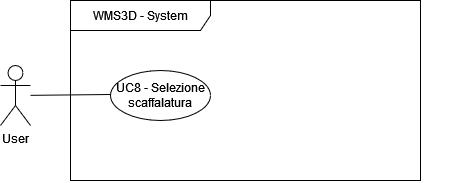
\includegraphics[width=0.8\textwidth]{UC_diagrams_1-10/UC8_sys.drawio.png}
   \caption{Diagramma UML UC8}
\end{figure}
\begin{figure}[H]
  \centering
  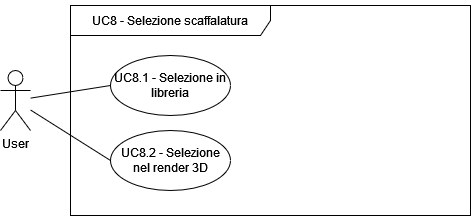
\includegraphics[width=0.8\textwidth]{UC_diagrams_1-10/UC8.drawio.png}
   \caption{Diagramma UML UC8 - dettaglio}
\end{figure}
\begin{itemize}
    \item \textbf{Attori:} User.
    \item \textbf{Pre-condizione:}  L'utente ha posizionato una scaffalatura [UC7] e la sta visualizzando nel render 3D [UC3.2] e nella libreria [UC4.1.1].
    \item \textbf{Post-condizione:} La scaffalatura presa in considerazione dall'utente viene selezionata ed evidenziata.
    \item \textbf{Scenario Principale:} L'utente seleziona la scaffalatura e, indipendentemente da dove la seleziona, questa verrà selezionata sia nella libreria [UC8.1] sia nel render 3D [UC8.2].
    \item \textbf{Generalizzazioni:} -
    \item \textbf{Estensioni:} -
\end{itemize}


\subsubsection{UC8.1 - Selezione scaffalatura in libreria}
\begin{figure}[H]
  \centering
  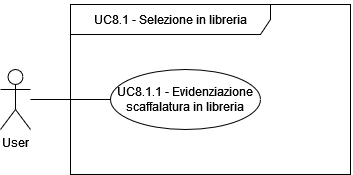
\includegraphics[width=0.8\textwidth]{UC_diagrams_1-10/UC8.1.drawio.png}
   \caption{Diagramma UML UC8.1}
\end{figure}
\begin{itemize}
    \item \textbf{Attori:} User.
    \item \textbf{Pre-condizione:} L'utente ha posizionato una scaffalatura [UC7] e la visualizza nella libreria [UC4.1.1].
    \item \textbf{Post-condizione:} La scaffalatura presa in considerazione dall'utente viene selezionata ed evidenziata nella libreria.
    \item \textbf{Scenario Principale:} L'utente seleziona la scaffalatura, la quale viene selezionata in libreria ed evidenziata in essa [UC8.1.1].
    \item \textbf{Generalizzazioni:} -
    \item \textbf{Estensioni:} -
\end{itemize}


\subsubsection{UC8.1.1 - Evidenziazione scaffalatura in libreria}
\begin{itemize}
    \item \textbf{Attori:} User.
    \item \textbf{Pre-condizione:} L'utente ha selezionato una scaffalatura [UC8].
    \item \textbf{Post-condizione:} La scaffalatura selezionata viene evidenziata in libreria.
    \item \textbf{Scenario Principale:} La scaffalatura selezionata viene evidenziata in libreria.
    \item \textbf{Generalizzazioni:} -
    \item \textbf{Estensioni:} -
\end{itemize}


\subsubsection{UC8.2 - Selezione scaffalatura in render 3D}
\begin{figure}[H]
  \centering
  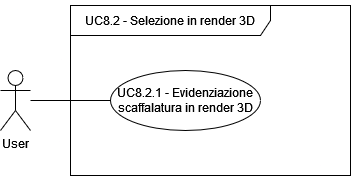
\includegraphics[width=0.8\textwidth]{UC_diagrams_1-10/UC8.2.drawio.png}
   \caption{Diagramma UML UC8.2}
\end{figure}
\begin{itemize}
    \item \textbf{Attori:} User.
    \item \textbf{Pre-condizione:} L'utente ha posizionato una scaffalatura [UC7] e la visualizza nel render 3D.
    \item \textbf{Post-condizione:} La scaffalatura presa in considerazione dall'utente viene selezionata ed evidenziata nel render 3D.
    \item \textbf{Scenario Principale:} L'utente seleziona la scaffalatura, la quale viene selezionata nel render 3D ed evidenziata in esso [UC8.2.1].
    \item \textbf{Generalizzazioni:} -
    \item \textbf{Estensioni:} -
\end{itemize}


\subsubsection{UC8.2.1 - Evidenziazione scaffalatura in render 3D}
\begin{itemize}
    \item \textbf{Attori:} User.
    \item \textbf{Pre-condizione:} L'utente ha selezionato una scaffalatura [UC8].
    \item \textbf{Post-condizione:} La scaffalatura selezionata viene evidenziata nel render 3D.
    \item \textbf{Scenario Principale:} La scaffalatura selezionata viene evidenziata nel render 3D.
    \item \textbf{Generalizzazioni:} -
    \item \textbf{Estensioni:} -
\end{itemize}
\subsection{UC9 - Modifica scaffalatura}
\begin{figure}[H]
  \centering
  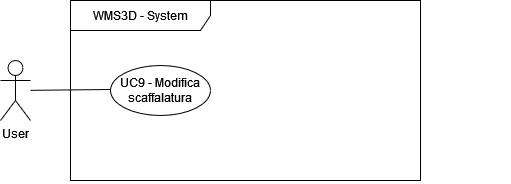
\includegraphics[width=0.8\textwidth]{UC_diagrams_1-10/UC9_sys.drawio.png}
   \caption{Diagramma UML UC9}
\end{figure}
\begin{figure}[H]
  \centering
  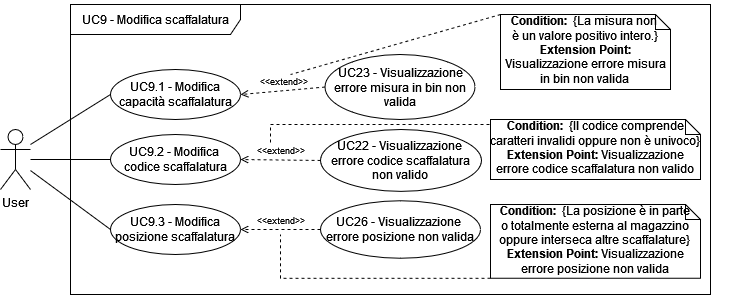
\includegraphics[width=0.8\textwidth]{UC_diagrams_1-10/UC9.drawio.png}
   \caption{Diagramma UML UC9 - dettaglio}
\end{figure}
\begin{itemize}
    \item \textbf{Attori:} User.
    \item \textbf{Pre-condizione:}  L'utente ha selezionato una scaffalatura [UC8].
    \item \textbf{Post-condizione:} La scaffalatura viene modificata.
    \item \textbf{Scenario Principale:} L'utente dopo aver selezionato una scaffalatura può modificarne le caratteristiche, in particolare può modificarne la capacità [UC9.1], il codice [UC9.2] oppure la posizione [UC9.3].
    \item \textbf{Generalizzazioni:} -
    \item \textbf{Estensioni:} -
\end{itemize}


\subsubsection{UC9.1 - Modifica capacità scaffalatura}
\begin{figure}[H]
  \centering
  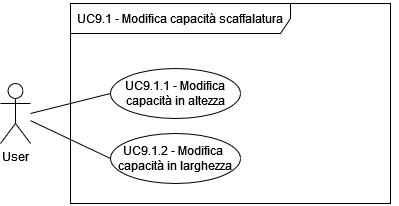
\includegraphics[width=0.8\textwidth]{UC_diagrams_1-10/UC9.1.drawio.png}
   \caption{Diagramma UML UC9.1}
\end{figure}
\begin{itemize}
    \item \textbf{Attori:} User.
    \item \textbf{Pre-condizione:}  L'utente ha selezionato una scaffalatura [UC8] e vuole modificarla.
    \item \textbf{Post-condizione:} Viene modificata la capacità della scaffalatura.
    \item \textbf{Scenario Principale:} L'utente dopo aver selezionato una scaffalatura può modificarne la capacità, in particolare può modificarne la capacità in altezza [UC9.1.1] oppure in larghezza [UC9.1.2].
    \item \textbf{Generalizzazioni:} -
    \item \textbf{Estensioni:} È presente una estensione:
    \begin{itemize}
        \item UC23 - Visualizzazione errore misura in bin non valida.
    \end{itemize}
\end{itemize}


\paragraph{UC9.1.1 - Modifica capacità in altezza}
\begin{figure}[H]
  \centering
  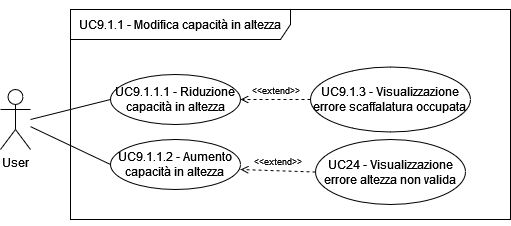
\includegraphics[width=0.8\textwidth]{UC_diagrams_1-10/UC9.1.1.drawio.png}
   \caption{Diagramma UML UC9.1.1}
\end{figure}
\begin{itemize}
    \item \textbf{Attori:} User.
    \item \textbf{Pre-condizione:} L'utente ha selezionato una scaffalatura [UC8] e vuole modificarne la capacità.
    \item \textbf{Post-condizione:} Viene modificata la capacità in altezza della scaffalatura.
    \item \textbf{Scenario Principale:} L'utente dopo aver selezionato una scaffalatura può modificarne l'altezza, in particolare può decide di ridurre [UC9.1.1.1] o aumentare [UC9.1.1.2] il numero di bin\textsuperscript{G} in altezza.
    \item \textbf{Generalizzazioni:} -
    \item \textbf{Estensioni:} -
\end{itemize}


\paragraph{UC9.1.1.1 - Riduzione capacità in altezza}
\begin{itemize}
    \item \textbf{Attori:} User.
    \item \textbf{Pre-condizione:} L'utente ha selezionato una scaffalatura [UC8] e vuole modificarne la capacità in altezza.
    \item \textbf{Post-condizione:} Viene diminuita la capacità in altezza della scaffalatura.
    \item \textbf{Scenario Principale:} L'utente dopo aver selezionato una scaffalatura può ridurre il numero di bin\textsuperscript{G} in altezza della scaffalatura.
    \item \textbf{Generalizzazioni:} -
    \item \textbf{Estensioni:} È presente una estensione:
    \begin{itemize}
        \item UC9.1.3 - Visualizzazione errore scaffalatura occupata.
    \end{itemize}
\end{itemize}


\paragraph{UC9.1.1.2 - Aumento capacità in altezza}
\begin{itemize}
    \item \textbf{Attori:} User.
    \item \textbf{Pre-condizione:} L'utente ha selezionato una scaffalatura [UC8] e vuole modificarne la capacità in altezza.
    \item \textbf{Post-condizione:} Viene aumentata la capacità in altezza della scaffalatura.
    \item \textbf{Scenario Principale:} L'utente dopo aver selezionato una scaffalatura può aumentare il numero di bin\textsuperscript{G} in altezza della scaffalatura.
    \item \textbf{Generalizzazioni:} -
    \item \textbf{Estensioni:} È presente una estensione:
    \begin{itemize}
        \item UC24 - Visualizzazione errore altezza non valida.
    \end{itemize}
\end{itemize}


\paragraph{UC9.1.2 - Modifica capacità in larghezza}
\begin{figure}[H]
  \centering
  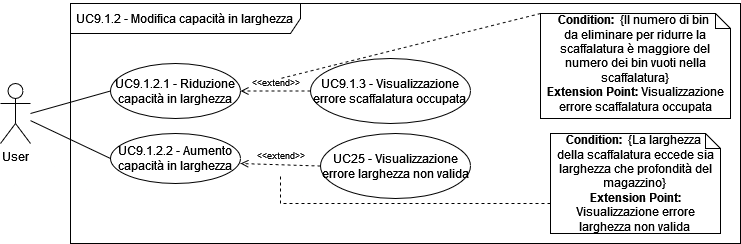
\includegraphics[width=0.8\textwidth]{UC_diagrams_1-10/UC9.1.2.drawio.png}
   \caption{Diagramma UML UC9.1.2}
\end{figure}
\begin{itemize}
    \item \textbf{Attori:} User.
    \item \textbf{Pre-condizione:} L'utente ha selezionato una scaffalatura [UC8] e vuole modificarne la capacità.
    \item \textbf{Post-condizione:} Viene modificata la capacità della scaffalatura.
    \item \textbf{Scenario Principale:} L'utente dopo aver selezionato una scaffalatura può modificarne l'altezza, in particolare può decide di ridurre [UC9.1.1.1] o aumentare [UC9.1.1.2] il numero di bin\textsuperscript{G} in larghezza.
    \item \textbf{Generalizzazioni:} -
    \item \textbf{Estensioni:} -
\end{itemize}


\paragraph{UC9.1.2.1 - Riduzione capacità in altezza}
\begin{itemize}
    \item \textbf{Attori:} User.
    \item \textbf{Pre-condizione:} L'utente ha selezionato una scaffalatura [UC8] e vuole modificarne la capacità in larghezza.
    \item \textbf{Post-condizione:} Viene diminuita la capacità in larghezza della scaffalatura.
    \item \textbf{Scenario Principale:} L'utente dopo aver selezionato una scaffalatura può ridurre il numero di bin\textsuperscript{G} in larghezza della scaffalatura.
    \item \textbf{Generalizzazioni:} -
    \item \textbf{Estensioni:} È presente una estensione:
    \begin{itemize}
        \item UC9.1.3 - Visualizzazione errore scaffalatura occupata.
    \end{itemize}
\end{itemize}


\paragraph{UC9.1.2.2 - Aumento capacità in larghezza}
\begin{itemize}
    \item \textbf{Attori:} User.
    \item \textbf{Pre-condizione:} L'utente ha selezionato una scaffalatura [UC8] e vuole modificarne la capacità in larghezza.
    \item \textbf{Post-condizione:} Viene aumentata la capacità in larghezza della scaffalatura.
    \item \textbf{Scenario Principale:} L'utente dopo aver selezionato una scaffalatura può aumentare il numero di bin\textsuperscript{G} in larghezza della scaffalatura.
    \item \textbf{Generalizzazioni:} -
    \item \textbf{Estensioni:} È presente una estensione:
    \begin{itemize}
        \item UC25 - Visualizzazione errore larghezza non valida.
    \end{itemize}
\end{itemize}


\paragraph{UC9.1.3 - Visualizzazione errore scaffalatura occupata}
\begin{itemize}
    \item \textbf{Attori:} User.
    \item \textbf{Pre-condizione:} Si desidera ridurre una scaffalatura, [UC9.1.1.1] o [UC9.1.2.1], per un numero di bin superiore al totale dei bin\textsuperscript{G} vuoti.
    \item \textbf{Post-condizione:} L'utente visualizza un messaggio d'errore e l'operazione fallisce.
    \item \textbf{Scenario Principale:} L'utente visualizza un messaggio informativo sull'errore e ne conferma la ricezione. L'operazione fallisce e l'utente dovrà quindi o spostare i prodotti presenti nei bin occupati oppure non ridurre di meno la scaffalatura.
    \item \textbf{Generalizzazioni:} -
    \item \textbf{Estensioni:} -
\end{itemize}


\subsubsection{UC9.2 - Modifica codice scaffalatura}
\begin{itemize}
    \item \textbf{Attori:} User.
    \item \textbf{Pre-condizione:} L'utente ha selezionato una scaffalatura [UC8] e vuole modificarla.
    \item \textbf{Post-condizione:} Viene modificato il codice della scaffalatura.
    \item \textbf{Scenario Principale:} L'utente dopo aver selezionato una scaffalatura può modificarne il codice.
    \item \textbf{Generalizzazioni:} -
    \item \textbf{Estensioni:} È presene una estensione:
    \begin{itemize}
        \item UC22 - Visualizzazione errore codice scaffalatura non valido.
    \end{itemize}
\end{itemize}


\subsubsection{UC9.3 - Modifica posizione scaffalatura}
\begin{itemize}
    \item \textbf{Attori:} User.
    \item \textbf{Pre-condizione:} L'utente ha selezionato una scaffalatura [UC8] e vuole modificarla.
    \item \textbf{Post-condizione:} Viene modificata la posizione della scaffalatura.
    \item \textbf{Scenario Principale:} L'utente dopo aver selezionato una scaffalatura può riposizionare la scaffalatura dove e come vuolte all'interno del magazzino.
    \item \textbf{Generalizzazioni:} -
    \item \textbf{Estensioni:} È presente una estensione:
    \begin{itemize}
        \item UC26 - Visualizzazione errore posizione non valida.
    \end{itemize}
\end{itemize}
\subsection{UC10 - Ricerca scaffalatura per codice}
\begin{figure}[H]
  \centering
  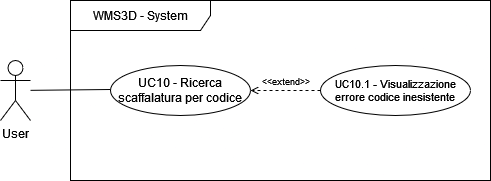
\includegraphics[width=0.8\textwidth]{UC_diagrams_1-10/UC10.drawio.png}
   \caption{Diagramma UML UC10}
\end{figure}
\begin{itemize}
    \item \textbf{Attori:} User.
    \item \textbf{Pre-condizione:} L'utente ha creato un magazzino [UC1].
    \item \textbf{Post-condizione:} L'utente può cercare una scaffalatura dando in input un codice e può visualizzarne i risultati [UC11].
    \item \textbf{Scenario Principale:} L'utente inserisce un codice per ricercare la scaffalatura corrispondente. I risultati della ricerca possono poi essere visualizzati [UC11].
    \item \textbf{Generalizzazioni:} -
    \item \textbf{Estensioni:} È presente una estensione:
    \begin{itemize}
        \item UC10.1 - Visualizzazione errore codice inesistente.
    \end{itemize}
\end{itemize}


\subsubsection{UC10.1 - Visualizzazione errore codice inesistente}
\begin{itemize}
    \item \textbf{Attori:} User.
    \item \textbf{Pre-condizione:}  L'utente ha inserito per la ricerca un codice che non corrisponde a nessuna scaffalatura.
    \item \textbf{Post-condizione:}  L'utente visualizza un messaggio d'errore e non sarà visualizzato nessun risultato per la ricerca.
    \item \textbf{Scenario Principale:}  L'utente visualizza un messaggio informativo sull'errore e ne conferma la ricezione. L'utente non visualizzerà alcun risultato della ricerca.
    \item \textbf{Generalizzazioni:} -
    \item \textbf{Estensioni:} -
\end{itemize}
\subsection{UC11 - Visualizzazione risultato ricerca scaffalatura}
\begin{figure}[H]
  \centering
  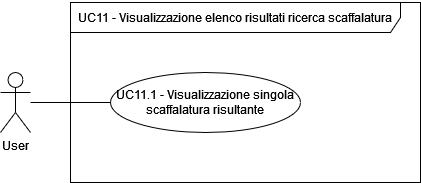
\includegraphics[width=0.8\textwidth]{UC_diagrams_11-20/UC11.drawio.png}
   \caption{Diagramma UML UC11 - Visualizzazione risultato ricerca scaffalatura}
\end{figure}
\begin{itemize}
    \item \textbf{Attori:} User.
    \item \textbf{Pre-condizione:} L'utente ha ricercato una scaffalatura [UC10].
    \item \textbf{Post-condizione:} La scaffalatura risultante dalla ricerca viene selezionata [UC8] all'interno di un elenco puntato/tabella nella libreria.
    \item \textbf{Scenario Principale:} L'utente, dopo aver ricercato un determinato codice, visualizza la scaffalatura corrispondente che verrà automaticamente selezionata.
    \item \textbf{Generalizzazioni:} -
    \item \textbf{Estensioni:} -
\end{itemize}
\subsection{UC12 - Cancellazione scaffalatura}
\begin{figure}[H]
  \centering
  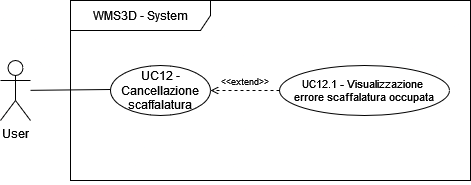
\includegraphics[width=0.8\textwidth]{UC_diagrams_11-20/UC12_sys.drawio.png}
   \caption{Diagramma UML UC12}
\end{figure}
\begin{figure}[H]
  \centering
  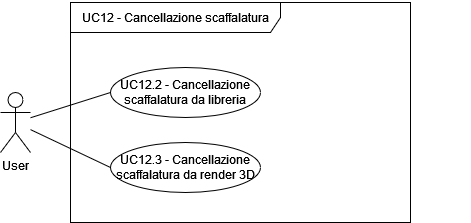
\includegraphics[width=0.8\textwidth]{UC_diagrams_11-20/UC12.drawio.png}
   \caption{Diagramma UML UC12 - dettaglio}
\end{figure}
\begin{itemize}
    \item \textbf{Attori:} User.
    \item \textbf{Pre-condizione:} L'utente ha selezionato una scaffalatura [UC8].
    \item \textbf{Post-condizione:} La scaffalatura viene eliminata.
    \item \textbf{Scenario Principale:} L'utente elimina da libreria [UC12.2] e dal render 3D [UC12.3] la scaffalatura precedentemente selezionata.
    \item \textbf{Generalizzazioni:} -
    \item \textbf{Estensioni:} È presente una estensione:
    \begin{itemize}
        \item UC12.1 - Visualizzazione errore scaffalatura occupata.
    \end{itemize}
\end{itemize}


\subsubsection{UC12.1 - Visualizzazione errore scaffalatura occupata}
\begin{itemize}
    \item \textbf{Attori:} User.
    \item \textbf{Pre-condizione:} L'utente vuole cancellare una scaffalatura [UC12] con prodotti posizionati all'interno.
    \item \textbf{Post-condizione:} L'utente visualizza un messaggio d'errore e l'operazione fallisce.
    \item \textbf{Scenario Principale:} L'utente visualizza un messaggio informativo sull'errore e ne conferma la ricezione. L'operazione fallisce e l'utente se vuole eliminare quella scaffalatura dovrà spostarne i prodotti.   
    \item \textbf{Generalizzazioni:} -
    \item \textbf{Estensioni:} -
\end{itemize}


\subsubsection{UC12.2 - Cancellazione scaffalatura da libreria}
\begin{itemize}
    \item \textbf{Attori:} User.
    \item \textbf{Pre-condizione:} L'utente ha selezionato una scaffalatura [UC8] e la vuole eliminare.
    \item \textbf{Post-condizione:} L'utente elimina la scaffalatura dalla libreria.
    \item \textbf{Scenario Principale:} L'utente elimina da libreria la scaffalatura precedentemente selezionata.   
    \item \textbf{Generalizzazioni:} -
    \item \textbf{Estensioni:} -
\end{itemize}


\subsubsection{UC12.3 - Cancellazione scaffalatura da render 3D}
\begin{itemize}
    \item \textbf{Attori:} User.
    \item \textbf{Pre-condizione:} L'utente ha selezionato una scaffalatura [UC8] e la vuole eliminare.
    \item \textbf{Post-condizione:} L'utente elimina la scaffalatura dal render 3D.
    \item \textbf{Scenario Principale:} L'utente elimina dal render 3D la scaffalatura precedentemente selezionata.   
    \item \textbf{Generalizzazioni:} -
    \item \textbf{Estensioni:} -
\end{itemize}
\subsection{UC13 - Creazione prodotto}
\begin{figure}[H]
  \centering
  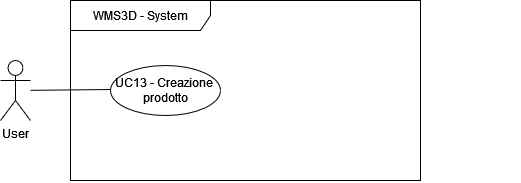
\includegraphics[width=0.8\textwidth]{UC_diagrams_11-20/UC13_sys.drawio.png}
   \caption{Diagramma UML UC13 - Creazione prodotto}
\end{figure}
\begin{figure}[H]
  \centering
  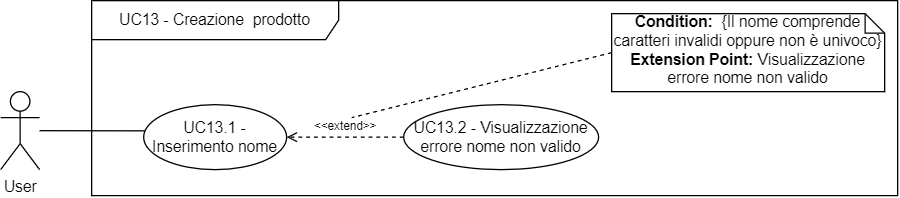
\includegraphics[width=0.8\textwidth]{UC_diagrams_11-20/UC13.drawio.png}
   \caption{Diagramma UML in dettaglio UC13 - Creazione prodotto}
\end{figure}
\begin{itemize}
    \item \textbf{Attori:} User.
    \item \textbf{Pre-condizione:}  L'utente ha creato/caricato un magazzino [UC1].
    \item \textbf{Post-condizione:} L'utente crea un prodotto che viene aggiunto in libreria.
    \item \textbf{Scenario Principale:}  L'utente crea un prodotto, inserendo un nome univoco [UC13.1] e delle dimensioni [UC13.2].
    \item \textbf{Generalizzazioni:} -
    \item \textbf{Estensioni:} -
\end{itemize}


\subsubsection{UC13.1 - Inserimento nome}
\begin{itemize}
    \item \textbf{Attori:} User.
    \item \textbf{Pre-condizione:}  L'utente ha creato/caricato un magazzino [UC1] e vuole creare un prodotto.
    \item \textbf{Post-condizione:} L'utente ha dato un nome identificativo al nuovo prodotto.
    \item \textbf{Scenario Principale:}  L'utente inserisce un nome univoco per il nuovo prodotto.
    \item \textbf{Generalizzazioni:} -
    \item \textbf{Estensioni:} È presente una estensione:
    \begin{itemize}
        \item UC13.3 - Visualizzazione errore nome non valido.
    \end{itemize}
\end{itemize}


\subsubsection{UC13.2 - Inserimento dimensioni}
\begin{figure}[H]
  \centering
  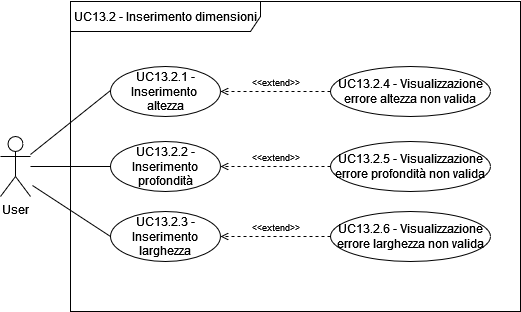
\includegraphics[width=0.8\textwidth]{UC_diagrams_11-20/UC13.2.drawio.png}
   \caption{Diagramma UML UC13.2 - Inserimento dimensioni}
\end{figure}
\begin{itemize}
    \item \textbf{Attori:} User.
    \item \textbf{Pre-condizione:}  L'utente ha creato/caricato un magazzino [UC1] e vuole creare un prodotto.
    \item \textbf{Post-condizione:} L'utente ha dato delle dimensioni al nuovo prodotto.
    \item \textbf{Scenario Principale:}  L'utente inserisce le dimensioni altezza [UC13.2.1], profondità [UC13.2.2] e larghezza [UC13.2.3] per il nuovo prodotto.
    \item \textbf{Generalizzazioni:} -
    \item \textbf{Estensioni:} -
\end{itemize}


\paragraph{UC13.2.1 - Inserimento altezza}
\begin{itemize}
    \item \textbf{Attori:} User.
    \item \textbf{Pre-condizione:}  L'utente ha creato/caricato un magazzino [UC1] e vuole creare un prodotto.
    \item \textbf{Post-condizione:} L'utente ha fornito l'altezza del nuovo prodotto.
    \item \textbf{Scenario Principale:}  L'utente inserisce l'altezza per il nuovo prodotto.
    \item \textbf{Generalizzazioni:} -
    \item \textbf{Estensioni:} È presente una estensione:
    \begin{itemize}
        \item UC13.2.4 - Visualizzazione errore altezza non valida.
    \end{itemize}
\end{itemize}


\paragraph{UC13.2.2 - Inserimento profondità}
\begin{itemize}
    \item \textbf{Attori:} User.
    \item \textbf{Pre-condizione:}  L'utente ha creato/caricato un magazzino [UC1] e vuole creare un prodotto.
    \item \textbf{Post-condizione:} L'utente ha fornito la profondità del nuovo prodotto.
    \item \textbf{Scenario Principale:}  L'utente inserisce la profondità per il nuovo prodotto.
    \item \textbf{Generalizzazioni:} -
    \item \textbf{Estensioni:} È presente una estensione:
    \begin{itemize}
        \item UC13.2.5 - Visualizzazione errore profondità non valida.
    \end{itemize}
\end{itemize}


\paragraph{UC13.2.3 - Inserimento larghezza}
\begin{itemize}
    \item \textbf{Attori:} User.
    \item \textbf{Pre-condizione:}  L'utente ha creato/caricato un magazzino [UC1] e vuole creare un prodotto.
    \item \textbf{Post-condizione:} L'utente ha fornito la larghezza del nuovo prodotto.
    \item \textbf{Scenario Principale:}  L'utente inserisce la larghezza per il nuovo prodotto.
    \item \textbf{Generalizzazioni:} -
    \item \textbf{Estensioni:} È presente una estensione:
    \begin{itemize}
        \item UC13.2.6 - Visualizzazione errore larghezza non valida.
    \end{itemize}
\end{itemize}


\paragraph{UC13.2.4 - Visualizzazione errore altezza non valida}
\begin{itemize}
    \item \textbf{Attori:} User.
    \item \textbf{Pre-condizione:}  L'altezza specificata del prodotto supera l'altezza del bin della scaffalatura.
    \item \textbf{Post-condizione:} L'utente visualizza un messaggio d'errore e l'operazione fallisce.
    \item \textbf{Scenario Principale:}  L'utente visualizza un messaggio informativo sull'errore e ne conferma la ricezione. L'operazione fallisce e l'utente dovrà scegliere una nuova altezza valida.
    \item \textbf{Generalizzazioni:} -
    \item \textbf{Estensioni:} -
\end{itemize}


\paragraph{UC13.2.5 - Visualizzazione errore profondità non valida}
\begin{itemize}
    \item \textbf{Attori:} User.
    \item \textbf{Pre-condizione:} La profondità specificata del prodotto supera la profondità del bin della scaffalatura.
    \item \textbf{Post-condizione:} L'utente visualizza un messaggio d'errore e l'operazione fallisce.
    \item \textbf{Scenario Principale:}  L'utente visualizza un messaggio informativo sull'errore e ne conferma la ricezione. L'operazione fallisce e l'utente dovrà scegliere una nuova profondità valida.
    \item \textbf{Generalizzazioni:} -
    \item \textbf{Estensioni:} -
\end{itemize}


\paragraph{UC13.2.5 - Visualizzazione errore larghezza non valida}
\begin{itemize}
    \item \textbf{Attori:} User.
    \item \textbf{Pre-condizione:}  La larghezza specificata del prodotto supera la larghezza del bin della scaffalatura.
    \item \textbf{Post-condizione:} L'utente visualizza un messaggio d'errore e l'operazione fallisce.
    \item \textbf{Scenario Principale:}  L'utente visualizza un messaggio informativo sull'errore e ne conferma la ricezione. L'operazione fallisce e l'utente dovrà scegliere una nuova larghezza valida.
    \item \textbf{Generalizzazioni:} -
    \item \textbf{Estensioni:} -
\end{itemize}


\subsubsection{UC13.3 - Visualizzazione errore nome non valido}
\begin{itemize}
    \item \textbf{Attori:} User.
    \item \textbf{Pre-condizione:}  L'utente ha inserito un nome identificativo di un prodotto che contiene caratteri invalidi oppure non è univoco.
    \item \textbf{Post-condizione:}  L'utente visualizza un messaggio d'errore e dovrà reinserire un nome diverso.
    \item \textbf{Scenario Principale:}  L'utente visualizza un messaggio informativo sull'errore e ne conferma la ricezione. L'operazione fallisce e l'utente dovrà scegliere un nuovo nome.
    \item \textbf{Generalizzazioni:} -
    \item \textbf{Estensioni:} -
\end{itemize}
\subsection{UC14 - Posizionamento prodotto in scaffalatura}
\begin{figure}[H]
  \centering
  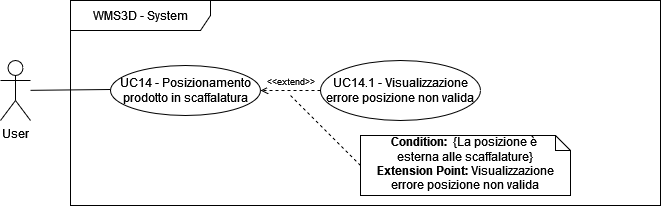
\includegraphics[width=0.8\textwidth]{UC_diagrams_11-20/UC14_sys.drawio.png}
   \caption{Diagramma UML UC14}
\end{figure}
\begin{figure}[H]
  \centering
  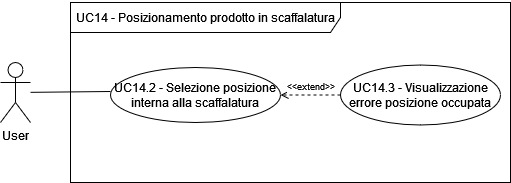
\includegraphics[width=0.8\textwidth]{UC_diagrams_11-20/UC14.drawio.png}
   \caption{Diagramma UML UC14 - dettaglio}
\end{figure}
\begin{itemize}
    \item \textbf{Attori:} User.
    \item \textbf{Pre-condizione:}  L'utente ha creato [UC6] e posizionato [UC7] una scaffalatura e ha creato anche un prodotto [UC13].
    \item \textbf{Post-condizione:} Il prodotto creato è posizionato nella scaffalatura creata presente all'interno del render 3D.
    \item \textbf{Scenario Principale:} L'utente dopo aver creato un prodotto sceglie in quale scaffalatura interna al magazzino posizionare il prodotto, e più specificatamente anche in quale bin interno posizionarlo [UC14.2].
    \item \textbf{Generalizzazioni:} -
    \item \textbf{Estensioni:} È presente una estensione nel caso in cui la posizione non sia valida:
    \begin{itemize}
        \item UC14.1 - Visualizzazione errore posizione non valida.
    \end{itemize}
\end{itemize}


\subsubsection{UC14.1 - Visualizzazione errore posizione non valida}
\begin{itemize}
    \item \textbf{Attori:} User.
    \item \textbf{Pre-condizione:}  L'utente cerca di posizionare il prodotto al di fuori delle scaffalature.
    \item \textbf{Post-condizione:} L'utente visualizza un messaggio d'errore e il posizionamento non viene permesso.
    \item \textbf{Scenario Principale:} L'utente visualizza un messaggio informativo sull'errore. L'utente dovrà cambiare posizionamento.
    \item \textbf{Generalizzazioni:} -
    \item \textbf{Estensioni:} -
\end{itemize}


\subsubsection{UC14.2 - Selezione posizione interna alla scaffalatura}
\begin{itemize}
    \item \textbf{Attori:} User.
    \item \textbf{Pre-condizione:}  L'utente ha creato [UC6] e posizionato [UC7] una scaffalatura e ha creato anche un prodotto [UC13]. 
    \item \textbf{Post-condizione:} Il prodotto creato è posizionato nel bin selezionato nella scaffalatura creata presente all'interno del render 3D.
    \item \textbf{Scenario Principale:} L'utente dopo aver creato un prodotto sceglie in quale bin\textsuperscript{G} e di quale scaffalatura posizionare il prodotto.
    \item \textbf{Generalizzazioni:} -
    \item \textbf{Estensioni:} È presente una estensione nel caso in cui il bin scelto sia occupato:
    \begin{itemize}
        \item UC14.3- Visualizzazione errore posizione occupata.
    \end{itemize}
\end{itemize}


\subsubsection{UC14.3 - Visualizzazione errore posizione occupata}
\begin{itemize}
    \item \textbf{Attori:} User.
    \item \textbf{Pre-condizione:}  L'utente cerca di posizionare il prodotto in un bin già occupato da un altro prodotto.
    \item \textbf{Post-condizione:} L'utente visualizza un messaggio d'errore e il posizionamento non viene permesso.
    \item \textbf{Scenario Principale:} L'utente visualizza un messaggio informativo sull'errore. L'utente dovrà cambiare posizionamento.
    \item \textbf{Generalizzazioni:} -
    \item \textbf{Estensioni:} -
\end{itemize}
\subsection{UC15 - Selezione prodotto}
\begin{figure}[H]
  \centering
  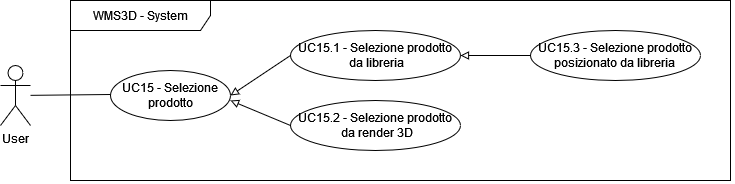
\includegraphics[width=0.8\textwidth]{UC_diagrams_11-20/UC15_sys.drawio.png}
   \caption{Diagramma UML UC15 - Selezione prodotto}
\end{figure}
\begin{itemize}
    \item \textbf{Attori:} User.
    \item \textbf{Pre-condizione:}  L'utente ha creato un prodotto [UC13].
    \item \textbf{Post-condizione:} Il prodotto preso in considerazione dall'utente viene selezionato da libreria o da render 3D.
    \item \textbf{Scenario Principale:} Il prodotto può essere selezionato dalla libreria [UC15.1] e, in tal caso, il prodotto verrà evidenziato in libreria [UC15.1.1] 
    e se il prodotto è posizionato [UC15.3] il prodotto verrà evidenziato anche nel render 3D [UC15.2.1.]. Se invece il prodotto è selezionato dal render 3D [15.2], sicuramente il prodotto è posizionato, e dunque sarà evidenziato su libreria [UC15.1.1] e render 3D [UC15.2.1.].
    \item \textbf{Generalizzazioni:} Sono presenti due generalizzazioni seconda del luogo in cui il prodotto viene selezionato:
    \begin{itemize}
        \item UC15.1 - Selezione prodotto da libreria;
        \item UC15.2 - Selezione prodotto da render 3D;
    \end{itemize}
    \item \textbf{Estensioni:} -
\end{itemize}


\subsubsection{UC15.1 - Selezione prodotto da libreria}
\begin{figure}[H]
  \centering
  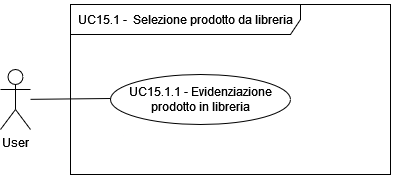
\includegraphics[width=0.8\textwidth]{UC_diagrams_11-20/UC15.1.drawio.png}
   \caption{Diagramma UML UC15.1 - Selezione prodotto da libreria}
\end{figure}
\begin{itemize}
    \item \textbf{Attori:} User.
    \item \textbf{Pre-condizione:}  L'utente ha creato un prodotto [UC13] e lo sta visualizzando nella libreria [UC4.2.1].
    \item \textbf{Post-condizione:} Il prodotto preso in considerazione dall'utente viene selezionato ed evidenziato in libreria.
    \item \textbf{Scenario Principale:} L'utente seleziona il prodotto dalla libreria e il prodotto verrà evidenziato in libreria [UC15.1.1].
    \item \textbf{Generalizzazioni:} È presente una generalizzazione nel caso in cui il prodotto sia posizionato nel magazzino 3D:
    \begin{itemize}
        \item UC15.3 - Selezione prodotto posizionato da libreria.
    \end{itemize}
    \item \textbf{Estensioni:} -
\end{itemize}


\paragraph{UC15.1.1 - Evidenziazione prodotto in libreria}
\begin{itemize}
    \item \textbf{Attori:} User.
    \item \textbf{Pre-condizione:}  L'utente ha selezionato un prodotto.
    \item \textbf{Post-condizione:} Il prodotto preso in considerazione dall'utente viene evidenziato nella libreria.
    \item \textbf{Scenario Principale:} L'utente seleziona il prodotto e questo viene evidenziato sempre nella libreria.
    \item \textbf{Generalizzazioni:} -
    \item \textbf{Estensioni:} -
\end{itemize}


\subsubsection{UC15.2 - Selezione prodotto da render 3D}
\begin{figure}[H]
  \centering
  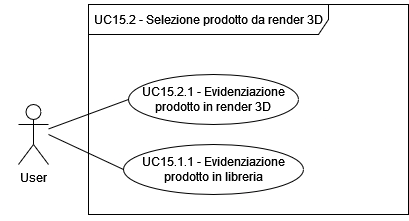
\includegraphics[width=0.8\textwidth]{UC_diagrams_11-20/UC15.2.drawio.png}
   \caption{Diagramma UML UC15.2 - Selezione prodotto da render 3D}
\end{figure}
\begin{itemize}
    \item \textbf{Attori:} User.
    \item \textbf{Pre-condizione:} L'utente ha creato un prodotto [UC13] e lo ha anche posizionato [UC14]. Al momento, lo sta visualizzando nella libreria [UC4.2.1] e nel render 3D [UC3.3].
    \item \textbf{Post-condizione:} Il prodotto preso in considerazione dall'utente viene selezionato dal render 3D ed evidenziato nel render 3D e nella libreria.
    \item \textbf{Scenario Principale:} L'utente seleziona il prodotto dal render 3D e questo verrà evidenziato nel render 3D [UC15.1.1.1] e nella libreria [15.2.1].
    \item \textbf{Generalizzazioni:} -
    \item \textbf{Estensioni:} -
\end{itemize}


\paragraph{UC15.2.1 - Evidenziazione prodotto in render 3D}
\begin{itemize}
    \item \textbf{Attori:} User.
    \item \textbf{Pre-condizione:} L'utente ha selezionato un prodotto posizionato nel render 3D.
    \item \textbf{Post-condizione:} Il prodotto preso in considerazione dall'utente viene evidenziato nel render 3D.
    \item \textbf{Scenario Principale:} L'utente seleziona il prodotto nel render 3D o nella libreria e questo viene evidenziato nel render 3D.
    \item \textbf{Generalizzazioni:} -
    \item \textbf{Estensioni:} -
\end{itemize}


\subsubsection{UC15.3 - Selezione prodotto posizionato da libreria}
\begin{figure}[H]
  \centering
  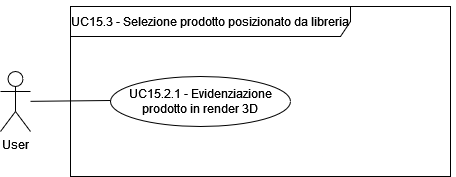
\includegraphics[width=0.8\textwidth]{UC_diagrams_11-20/UC15.3.drawio.png}
   \caption{Diagramma UML UC15.3 - Selezione prodotto posizionato da libreria}
\end{figure}
\begin{itemize}
    \item \textbf{Attori:} User.
    \item \textbf{Pre-condizione:} L'utente ha creato un prodotto [UC13] e lo ha anche posizionato [UC14]. Al momento, lo sta visualizzando nella libreria [UC4.2.1] e nel render 3D [UC3.3].
    \item \textbf{Post-condizione:} Il prodotto preso in considerazione dall'utente viene selezionato dalla libreria ed evidenziato in libreria e nel render 3D.
    \item \textbf{Scenario Principale:} Il prodotto viene selezionato dalla libreria, però questo essendo posizionato, verrà evidenziato sia nella libreria [UC15.1.1] sia nel render 3D [UC15.2.1].
    \item \textbf{Generalizzazioni:} -
    \item \textbf{Estensioni:} -
\end{itemize}


\subsection{UC16 - Ricerca prodotto per nome}
\begin{figure}[H]
  \centering
  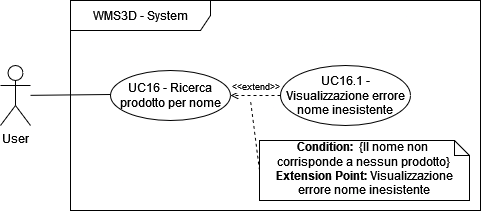
\includegraphics[width=0.8\textwidth]{UC_diagrams_11-20/UC16.drawio.png}
   \caption{Diagramma UML UC16 - Ricerca prodotto per nome}
\end{figure}
\begin{itemize}
    \item \textbf{Attori:} User.
    \item \textbf{Pre-condizione:} L'utente ha creato un magazzino [UC1].
    \item \textbf{Post-condizione:} L'utente può cercare un prodotto dando in input un nome e può visualizzarne i risultati [UC17].
    \item \textbf{Scenario Principale:} L'utente inserisce un nome per ricercare il prodotto corrispondente. I risultati della ricerca possono poi essere visualizzati [UC17].
    \item \textbf{Generalizzazioni:} -
    \item \textbf{Estensioni:} È presente una estensione:
    \begin{itemize}
        \item UC16.1 - Visualizzazione errore nome inesistente.
    \end{itemize}
\end{itemize}


\subsubsection{UC16.1 - Visualizzazione errore codice inesistente}
\begin{itemize}
    \item \textbf{Attori:} User.
    \item \textbf{Pre-condizione:}  L'utente ha inserito per la ricerca un nome che non corrisponde a nessun prodotto.
    \item \textbf{Post-condizione:}  L'utente visualizza un messaggio d'errore e non sarà visualizzato nessun risultato per la ricerca.
    \item \textbf{Scenario Principale:}  L'utente visualizza un messaggio informativo sull'errore e ne conferma la ricezione. L'utente non visualizzerà alcun risultato della ricerca.
    \item \textbf{Generalizzazioni:} -
    \item \textbf{Estensioni:} -
\end{itemize}
\subsection{UC17 - Visualizzazione risultato ricerca prodotto}
\begin{figure}[H]
  \centering
  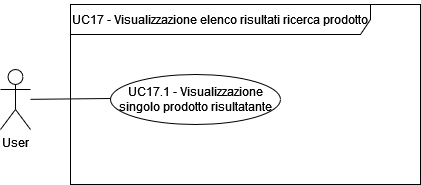
\includegraphics[width=0.8\textwidth]{UC_diagrams_11-20/UC17.drawio.png}
   \caption{Diagramma UML UC17 - Visualizzazione risultato ricerca prodotto}
\end{figure}
\begin{itemize}
    \item \textbf{Attori:} User.
    \item \textbf{Pre-condizione:} L'utente ha ricercato un prodotto [UC16].
    \item \textbf{Post-condizione:} Il prodotto risultante dalla ricerca viene selezionato [UC15], all'interno di un elenco puntato/tabella nella libreria.
    \item \textbf{Scenario Principale:} L'utente, dopo aver ricercato un determinato nome, visualizza il prodotto corrispondente che verrà automaticamente selezionato.
    \item \textbf{Generalizzazioni:} -
    \item \textbf{Estensioni:} -
\end{itemize}
\subsection{UC18 - Cancellazione prodotto}
\begin{figure}[H]
  \centering
  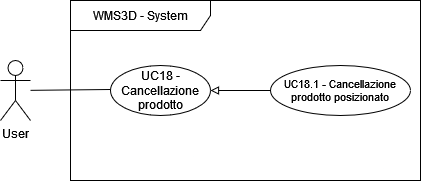
\includegraphics[width=0.8\textwidth]{UC_diagrams_11-20/UC18_sys.drawio.png}
   \caption{Diagramma UML UC18}
\end{figure}
\begin{figure}[H]
  \centering
  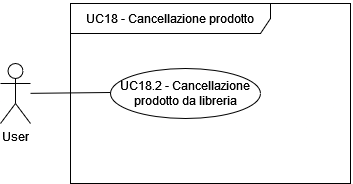
\includegraphics[width=0.8\textwidth]{UC_diagrams_11-20/UC18.drawio.png}
   \caption{Diagramma UML UC18 - dettaglio}
\end{figure}
\begin{itemize}
    \item \textbf{Attori:} User.
    \item \textbf{Pre-condizione:} L'utente ha selezionato un prodotto [UC15].
    \item \textbf{Post-condizione:} Il prodotto viene eliminato dalla libreria e dal render 3D.
    \item \textbf{Scenario Principale:} L'utente elimina da libreria [UC18.2] il prodotto precedentemente selezionato. Se il prodotto era stato posizionato [UC18.1], lo elimina anche dal render 3D [UC18.1.1].
    \item \textbf{Generalizzazioni:} È presente una generalizzazione in caso in cui il prodotto sia stato posizionato:
    \begin{itemize}
        \item UC18.1 - Cancellazione prodotto posizionato.
    \end{itemize}
    \item \textbf{Estensioni:} -
\end{itemize}


\subsubsection{UC18.1 - Cancellazione prodotto posizionato}
\begin{figure}[H]
  \centering
  \includegraphics[width=0.8\textwidth]{UC_diagrams_11-20/UC18.1.drawio.png}
   \caption{Diagramma UML UC18.1}
\end{figure}
\begin{itemize}
    \item \textbf{Attori:} User.
    \item \textbf{Pre-condizione:} L'utente ha selezionato un prodotto [UC15] che è stato posizionato [UC14] e lo vuole eliminare.
    \item \textbf{Post-condizione:} L'utente elimina il prodotto dalla libreria e dal render 3D.
    \item \textbf{Scenario Principale:} L'utente elimina dalla libreria [UC18.2] e dal render 3D [UC18.1.1] il prodotto precedentemente selezionato.   
    \item \textbf{Generalizzazioni:} -
    \item \textbf{Estensioni:} -
\end{itemize}


\paragraph{UC18.1.1 - Cancellazione prodotto da render 3D}
\begin{itemize}
    \item \textbf{Attori:} User.
    \item \textbf{Pre-condizione:} L'utente ha selezionato un prodotto [UC15] che è stato posizionato [UC14] e lo vuole eliminare.
    \item \textbf{Post-condizione:} L'utente elimina il prodotto dal render 3D.
    \item \textbf{Scenario Principale:} L'utente elimina dal render 3D il prodotto posizionato precedentemente selezionato.   
    \item \textbf{Generalizzazioni:} -
    \item \textbf{Estensioni:} -
\end{itemize}


\subsubsection{UC18.2 - Cancellazione prodotto da libreria}
\begin{itemize}
    \item \textbf{Attori:} User.
    \item \textbf{Pre-condizione:} L'utente ha selezionato un prodotto [UC15] e lo vuole eliminare.
    \item \textbf{Post-condizione:} L'utente elimina il prodotto dalla libreria.
    \item \textbf{Scenario Principale:} L'utente elimina da libreria il prodotto precedentemente selezionato.   
    \item \textbf{Generalizzazioni:} -
    \item \textbf{Estensioni:} -
\end{itemize}
\subsection{UC19 - Richiesta di spostamento}
\begin{figure}[H]
  \centering
  \includegraphics[width=0.8\textwidth]{UC_diagrams_11-20/UC19_sys.drawio.png}
   \caption{Diagramma UML UC19}
\end{figure}
\begin{figure}[H]
  \centering
  \includegraphics[width=0.8\textwidth]{UC_diagrams_11-20/UC19.drawio.png}
   \caption{Diagramma UML UC19 - dettaglio}
\end{figure}
\begin{itemize}
    \item \textbf{Attori:} User.
    \item \textbf{Pre-condizione:} L'utente ha selezionato un prodotto [UC15] che è stato posizionato [UC14].
    \item \textbf{Post-condizione:} L'utente richiede lo spostamento del prodotto.
    \item \textbf{Scenario Principale:} L'utente seleziona la destinazione per la movimentazione del prodotto [UC19.1] e si richiede lo spostamento.  
    \item \textbf{Generalizzazioni:} -
    \item \textbf{Estensioni:} -
\end{itemize}


\subsubsection{UC19.1 - Selezione scaffalatura di destinazione}
\begin{figure}[H]
  \centering
  \includegraphics[width=0.8\textwidth]{UC_diagrams_11-20/UC19.1.drawio.png}
   \caption{Diagramma UML UC19.1}
\end{figure}
\begin{itemize}
    \item \textbf{Attori:} User.
    \item \textbf{Pre-condizione:} L'utente vuole richiedere lo spostamento di un prodotto [UC19].
    \item \textbf{Post-condizione:} Viene selezionata la destinazione dello spostamento.
    \item \textbf{Scenario Principale:} L'utente seleziona la scaffalatura, e in particolar modo il bin\textsuperscript{G} [UC19.1.1], di destinazione della movimentazione del prodotto.
    \item \textbf{Generalizzazioni:} -
    \item \textbf{Estensioni:} È presente una estensione:
    \begin{itemize}
        \item UC19.2 - Visualizzazione errore destinazione non valida.
    \end{itemize}
\end{itemize}


\paragraph{UC19.1.1 - Selezione posizione interna alla scaffalatura}
\begin{itemize}
    \item \textbf{Attori:} User.
    \item \textbf{Pre-condizione:}  L'utente vuole richiedere lo spostamento di un prodotto [UC19].
    \item \textbf{Post-condizione:} Viene selezionato il bin\textsuperscript{G} interno alla scaffalatura come destinazione dello spostamento.
    \item \textbf{Scenario Principale:} L'utente dopo aver creato un prodotto sceglie a quale bin\textsuperscript{G} destinare il prodotto.
    \item \textbf{Generalizzazioni:} -
    \item \textbf{Estensioni:} È presente una estensione nel caso in cui il bin\textsuperscript{G} scelto sia occupato:
    \begin{itemize}
        \item UC19.1.2- Visualizzazione errore posizione occupata.
    \end{itemize}
\end{itemize}


\paragraph{UC19.1.2 - Visualizzazione errore posizione occupata}
\begin{itemize}
    \item \textbf{Attori:} User.
    \item \textbf{Pre-condizione:}  L'utente cerca di destinare lo spostamento del prodotto ad un bin già occupato da un altro prodotto.
    \item \textbf{Post-condizione:} L'utente visualizza un messaggio d'errore e la richiesta non viene inoltrata.
    \item \textbf{Scenario Principale:} L'utente visualizza un messaggio informativo sull'errore. L'utente dovrà cambiare destinazione.
    \item \textbf{Generalizzazioni:} -
    \item \textbf{Estensioni:} -
\end{itemize}


\subsubsection{UC19.2 - Visualizzazione errore destinazione non valida}
\begin{itemize}
    \item \textbf{Attori:} User.
    \item \textbf{Pre-condizione:}  L'utente cerca di destinare il prodotto in una posizione al di fuori delle scaffalature.
    \item \textbf{Post-condizione:} L'utente visualizza un messaggio d'errore e il posizionamento non viene permesso.
    \item \textbf{Scenario Principale:} L'utente visualizza un messaggio informativo sull'errore. L'utente dovrà cambiare destinazione.
    \item \textbf{Generalizzazioni:} -
    \item \textbf{Estensioni:} -
\end{itemize}
\subsection{UC20 - Visualizzazione richieste di spostamento pendenti}
\begin{figure}[H]
  \centering
  \includegraphics[width=0.8\textwidth]{UC_diagrams_11-20/UC20_sys.drawio.png}
   \caption{Diagramma UML UC20}
\end{figure}
\begin{figure}[H]
  \centering
  \includegraphics[width=0.8\textwidth]{UC_diagrams_11-20/UC20.drawio.png}
   \caption{Diagramma UML UC20 - dettaglio}
\end{figure}
\begin{itemize}
    \item \textbf{Attori:} User.
    \item \textbf{Pre-condizione:}  L'utente ha richiesto lo spostamento di un prodotto [UC19].
    \item \textbf{Post-condizione:} Si visualizzano tutte le richieste di spostamento inoltrate.
    \item \textbf{Scenario Principale:} L'utente dopo aver richiesto lo spostamento di un prodotto, può visualizzare per ogni richiesta i dettagli ad essa relativa [UC20.1].
    \item \textbf{Generalizzazioni:} -
    \item \textbf{Estensioni:} -
\end{itemize}


\subsubsection{UC20.1 - Visualizzazione singola richiesta di spostamento pendente}
\begin{figure}[H]
  \centering
  \includegraphics[width=0.8\textwidth]{UC_diagrams_11-20/UC20.1.drawio.png}
   \caption{Diagramma UML UC20.1}
\end{figure}
\begin{itemize}
    \item \textbf{Attori:} User.
    \item \textbf{Pre-condizione:}  L'utente ha richiesto lo spostamento di un prodotto [UC19] e vuole visualizzare lo stato della richiesta.
    \item \textbf{Post-condizione:} Si visualizza i dettagli della singola richiesta di spostamento.
    \item \textbf{Scenario Principale:} Per ogni singola richiesta di spostamento si visualizzano il nome [UC20.1.1], la posizione d'origine [UC20.1.2] e di destinazione [UC20.1.3] del prodotto oggetto della richiesta.
    \item \textbf{Generalizzazioni:} -
    \item \textbf{Estensioni:} -
\end{itemize}


\paragraph{UC20.1.1 - Visualizzazione nome prodotto}
\begin{itemize}
    \item \textbf{Attori:} User.
    \item \textbf{Pre-condizione:}  L'utente sta visualizzando una richiesta di spostamento.
    \item \textbf{Post-condizione:} L'utente visualizza il nome del prodotto.
    \item \textbf{Scenario Principale:} Per ogni singola richiesta di spostamento l'utente visualizza il nome del prodotto oggetto della richiesta.
    \item \textbf{Generalizzazioni:} -
    \item \textbf{Estensioni:} -
\end{itemize}


\paragraph{UC20.1.2 - Visualizzazione posizione origine prodotto}
\begin{itemize}
    \item \textbf{Attori:} User.
    \item \textbf{Pre-condizione:}  L'utente sta visualizzando una richiesta di spostamento.
    \item \textbf{Post-condizione:} L'utente visualizza la posizione originale del prodotto.
    \item \textbf{Scenario Principale:} Per ogni singola richiesta di spostamento l'utente visualizza la posizione originale del prodotto oggetto della richiesta.
    \item \textbf{Generalizzazioni:} -
    \item \textbf{Estensioni:} -
\end{itemize}


\paragraph{UC20.1.3 - Visualizzazione posizione destinazione prodotto}
\begin{itemize}
    \item \textbf{Attori:} User.
    \item \textbf{Pre-condizione:}  L'utente sta visualizzando una richiesta di spostamento.
    \item \textbf{Post-condizione:} L'utente visualizza la posizione di destinazione del prodotto.
    \item \textbf{Scenario Principale:} Per ogni singola richiesta di spostamento l'utente visualizza la posizione di destinazione del prodotto oggetto della richiesta.
    \item \textbf{Generalizzazioni:} -
    \item \textbf{Estensioni:} -
\end{itemize}
\subsection{UC21 - Visualizzazione errore inserimento misura}
\begin{figure}[H]
  \centering
  \includegraphics[width=0.8\textwidth]{UC_diagrams_21-26/UC21.drawio.png}
   \caption{Diagramma UML UC21}
\end{figure}
\begin{itemize}
    \item \textbf{Attori:} User.
    \item \textbf{Pre-condizione:}  L'utente ha inserito in un dato di tipo misura un valore non compreso tra i valori numerici positivi razionali.
    \item \textbf{Post-condizione:} L'utente visualizza un messaggio d'errore e l'operazione fallisce.
    \item \textbf{Scenario Principale:}  L'utente visualizza un messaggio informativo sull'errore e ne conferma la ricezione. L'operazione, di conseguenza, fallisce.
    \item \textbf{Generalizzazioni:} -
    \item \textbf{Estensioni:} -
\end{itemize}
\subsection{UC22 - Visualizzazione errore codice scaffalatura non valido}
\begin{figure}[H]
  \centering
  \includegraphics[width=0.8\textwidth]{UC_diagrams_21-26/UC22.drawio.png}
   \caption{Diagramma UML UC22 - Visualizzazione errore codice scaffalatura non valido}
\end{figure}
\begin{itemize}
    \item \textbf{Attori:} User.
    \item \textbf{Pre-condizione:}  L'utente ha inserito un codice identificativo di una scaffalatura che contiene caratteri invalidi oppure non è univoco.
    \item \textbf{Post-condizione:}  L'utente visualizza un messaggio d'errore e dovrà reinserire un codice diverso.
    \item \textbf{Scenario Principale:}  L'utente visualizza un messaggio informativo sull'errore e ne conferma la ricezione. L'operazione fallisce e l'utente dovrà scegliere un nuovo codice.
    \item \textbf{Generalizzazioni:} -
    \item \textbf{Estensioni:} -
\end{itemize}
\subsection{UC23 - Visualizzazione errore misura in bin non valida}
\begin{figure}[H]
  \centering
  \includegraphics[width=0.8\textwidth]{UC_diagrams_21-27/UC23.drawio.png}
   \caption{Diagramma UML UC23 - Visualizzazione errore misura in bin non valida}
\end{figure}
\begin{itemize}
    \item \textbf{Attori:} User.
    \item \textbf{Pre-condizione:}  L'utente ha inserito in un dato di tipo misura in bin un valore non compreso tra i valori numerici positivi interi.
    \item \textbf{Post-condizione:} L'utente visualizza un messaggio d'errore e l'operazione fallisce.
    \item \textbf{Scenario Principale:}  L'utente visualizza un messaggio informativo sull'errore e ne conferma la ricezione. L'operazione, di conseguenza, fallisce.
    \item \textbf{Generalizzazioni:} -
    \item \textbf{Estensioni:} -
\end{itemize}
\subsection{UC24 - Visualizzazione errore altezza non valida}
\begin{figure}[H]
  \centering
  \includegraphics[width=0.8\textwidth]{UC_diagrams_21-27/UC24.drawio.png}
   \caption{Diagramma UML UC24 - Visualizzazione errore altezza non valida}
\end{figure}
\begin{itemize}
    \item \textbf{Attori:} User.
    \item \textbf{Pre-condizione:}  La capacità in altezza della scaffalatura inserita supera l'altezza complessiva del magazzino.
    \item \textbf{Post-condizione:} L'utente visualizza un messaggio d'errore e l'operazione fallisce.
    \item \textbf{Scenario Principale:}  L'utente visualizza un messaggio informativo sull'errore e ne conferma la ricezione. L'operazione fallisce e l'utente dovrà scegliere una nuova altezza valida.
    \item \textbf{Generalizzazioni:} -
    \item \textbf{Estensioni:} -
\end{itemize}
\subsection{UC25 - Visualizzazione errore larghezza non valida}
\begin{figure}[H]
  \centering
  \includegraphics[width=0.8\textwidth]{UC_diagrams_21-27/UC25.drawio.png}
   \caption{Diagramma UML UC25 - Visualizzazione errore larghezza non valida}
\end{figure}
\begin{itemize}
    \item \textbf{Attori:} User.
    \item \textbf{Pre-condizione:}  La capacità in larghezza supera sia larghezza che profondità complessiva del magazzino.
    \item \textbf{Post-condizione:} L'utente visualizza un messaggio d'errore e l'operazione fallisce.
    \item \textbf{Scenario Principale:}  L'utente visualizza un messaggio informativo sull'errore e ne conferma la ricezione. L'operazione fallisce e l'utente dovrà scegliere una nuova larghezza valida.
    \item \textbf{Generalizzazioni:} -
    \item \textbf{Estensioni:} -
\end{itemize}
\subsection{UC26 - Visualizzazione errore posizione non valida}
\begin{figure}[H]
  \centering
  \includegraphics[width=0.8\textwidth]{UC_diagrams_21-26/UC26.drawio.png}
   \caption{Diagramma UML UC26}
\end{figure}
\begin{itemize}
    \item \textbf{Attori:} User.
    \item \textbf{Pre-condizione:}  L'utente sceglie una posizione per la scaffalatura che eccede i confini del magazzino o che interseca altre scaffalature.
    \item \textbf{Post-condizione:} L'utente visualizza un messaggio d'errore e il posizionamento non viene permesso.
    \item \textbf{Scenario Principale:} L'utente visualizza un messaggio informativo sull'errore. L'utente dovrà cambiare posizionamento.
    \item \textbf{Generalizzazioni:} -
    \item \textbf{Estensioni:} -
\end{itemize}
\subsection{UC27 - Visualizzazione errore dimensioni bin non valide}
\begin{figure}[H]
  \centering
  \includegraphics[width=0.8\textwidth]{UC_diagrams_21-27/UC27.drawio.png}
  \caption{Diagramma UML UC26 - Visualizzazione errore posizione non valida}
\end{figure}
\begin{itemize}
    \item \textbf{Attori:} User.
    \item \textbf{Pre-condizione:}  L'utente sceglie una dimensione per il bin della scaffalatura che eccede i confini del magazzino o che è più piccola delle dimensioni minime previste.
    \item \textbf{Post-condizione:} L'utente visualizza un messaggio d'errore e le dimensioni del bin non vengono inserite.
    \item \textbf{Scenario Principale:} L'utente visualizza un messaggio informativo sull'errore.
    \item \textbf{Generalizzazioni:} -
    \item \textbf{Estensioni:} -
\end{itemize}
\subsection{UC28 - Suddivisione Planimetria}
\begin{figure}[H]
  \centering
  \includegraphics[width=0.8\textwidth]{UC_diagrams_21-27/UC28.drawio.png}
  \caption{Diagramma UML UC28 - Suddivisione Planimetria}
\end{figure}
\begin{itemize}
    \item \textbf{Attori:} User.
    \item \textbf{Pre-condizione:}  Il sistema é istanziato correttamente.
    \item \textbf{Post-condizione:} L'utente ha effettuato una modifica alla suddivisione del magazzino.
    \item \textbf{Scenario Principale:} L'utente entra nella schermata di suddivisione della planimetria e sceglie un'azione da compiere tra: Inserimento nuova suddivisione [UC28.1], Eliminazione suddivisione [UC28.2] e Modifica Suddivisione[UC28.3]. Le suddivisioni dividono il magazzino in zone adibite ad uno scopo evidenziandone la diversitá nell'ambiente 3D.
    \item \textbf{Generalizzazioni:} Sono presenti 3 Generalizzazioni:
        \begin{itemize}
        \item UC28.1 Inserimento nuova Suddivisone
        \item UC28 Eliminazione Suddivisione
        \item UC28.3 Modifica Suddivisione
    \end{itemize}
    \item \textbf{Estensioni:} -
\end{itemize}

\subsection{UC28.1 - Inserimento nuova suddivisione}
\begin{figure}[H]
  \centering
  \includegraphics[width=0.8\textwidth]{UC_diagrams_21-27/UC28.1.drawio.png}
  \caption{Diagramma UML UC28.1 - Inserimento nuova suddivisione}
\end{figure}
\begin{itemize}
    \item \textbf{Attori:} User.
    \item \textbf{Pre-condizione:}  Il sistema é istanziato correttamente. L'utente ha scelto di inserire una nuova suddivisione della planimetria.
    \item \textbf{Post-condizione:} L'utente ha inserito correttamente una nuova suddivisione o ha annullato l'operazione.
    \item \textbf{Scenario Principale:} L'utente crea una nuova suddivisione scegliendone dapprima la posizione [UC28.1.1] e poi il tag [UC28.1.2]
    \item \textbf{Generalizzazioni:} -
    \item \textbf{Estensioni:} -
\end{itemize}

\subsection{UC28.1.1 - Selezione Posizione}
\begin{itemize}
    \item \textbf{Attori:} User.
    \item \textbf{Pre-condizione:}  L'utente è nella schermata di inserimento di una nuova suddivisione.
    \item \textbf{Post-condizione:} L'utente ha inserito la posizione della nuova suddivisione.
    \item \textbf{Scenario Principale:} L'utente sceglie una posizione per la nuova suddivisione all'interno della planimetria.
    \item \textbf{Estensioni:} -
\end{itemize}

\subsection{UC28.1.2 - Inserimento Tag}
\begin{itemize}
    \item \textbf{Attori:} User.
    \item \textbf{Pre-condizione:}  L'utente ha scelto una posizione per la nuova suddivisione.
    \item \textbf{Post-condizione:} L'utente ha inserito corretamente un Tag.
    \item \textbf{Scenario Principale:} L'utente sceglie un nome per la nuova suddivisione.
    \item \textbf{Generalizzazioni:} -
    \item \textbf{Estensioni:} -
\end{itemize}

\subsection{UC28.2 - Eliminazione suddivisione}
\begin{itemize}
    \item \textbf{Attori:} User.
    \item \textbf{Pre-condizione:}  L'utente è nella schermata di suddivisione planimetria.
    \item \textbf{Post-condizione:} L'utente ha eliminato una suddivisione o ha annullato.
    \item \textbf{Scenario Principale:} L'utente selezione una suddivisione e la elimina, oppure annulla il processo.
    \item \textbf{Generalizzazioni:} -
    \item \textbf{Estensioni:} -
\end{itemize}

\subsection{UC28.3 - Modifica suddivisione}
\begin{figure}[H]
  \centering
  \includegraphics[width=0.8\textwidth]{UC_diagrams_21-27/UC28.3.drawio.png}
  \caption{Diagramma UML UC28.3 - Modifica suddivisione}
\end{figure}
\begin{itemize}
    \item \textbf{Attori:} User.
    \item \textbf{Pre-condizione:}  Il sistema é istanziato correttamente. L'utente ha scelto di modificare una suddivisione della planimetria.
    \item \textbf{Post-condizione:} L'utente ha modificato correttamente una nuova suddivisione o ha annullato l'operazione.
    \item \textbf{Scenario Principale:} L'utente modifica la posizione [UC28.3.1] o il tag [28.3.2] di una suddivisione
    \item \textbf{Generalizzazioni:} Sono presenti due generalizzazioni:
    \begin{itemize}
        \item UC28.3.1 Modifica Posizione
        \item UC28.3.2 Modifica Tag
    \end{itemize}
    \item \textbf{Estensioni:} -
\end{itemize}

\subsection{UC28.1.1 - Modifica Posizione}
\begin{itemize}
    \item \textbf{Attori:} User.
    \item \textbf{Pre-condizione:}  L'utente è nella schermata di modifica di una  suddivisione.
    \item \textbf{Post-condizione:} L'utente ha modifica la posizione della suddivisione.
    \item \textbf{Scenario Principale:} L'utente sceglie una nuova posizione per la suddivisione all'interno della planimetria.
    \item \textbf{Estensioni:} -
\end{itemize}

\subsection{UC28.1.2 - Modifica Tag}
\begin{itemize}
    \item \textbf{Attori:} User.
    \item \textbf{Pre-condizione:}  L'utente è nella schermata di modifica di una  suddivisione.
    \item \textbf{Post-condizione:} L'utente ha inserito corretamente un nuovo Tag.
    \item \textbf{Scenario Principale:} L'utente sceglie un nuovo nome per la suddivisione.
    \item \textbf{Generalizzazioni:} -
    \item \textbf{Estensioni:} -
\end{itemize}


\subsection{UC29 - Visualizzazione Errore Posizione}
\begin{itemize}
    \item \textbf{Attori:} User.
    \item \textbf{Pre-condizione:}  L'utente è nella schermata di modifica di una  suddivisione ed ha inserito una posizione per una suddivisione.
    \item \textbf{Post-condizione:} L'utente visualizza un messaggio di errore.
    \item \textbf{Scenario Principale:} L'utente ha scelto una posizione scorretta e visualizza un messaggio di errore corrispondente.
    \item \textbf{Generalizzazioni:} -
    \item \textbf{Estensioni:} -
\end{itemize}
\subsection{UC30 - Visualizzazione Errore tag}
\begin{itemize}
    \item \textbf{Attori:} User.
    \item \textbf{Pre-condizione:}  L'utente è nella schermata di modifica di una  suddivisione ed ha inserito un Tag per una suddivisione.
    \item \textbf{Post-condizione:} L'utente visualizza un messaggio di errore.
    \item \textbf{Scenario Principale:} L'utente ha scelto un Tag scorretto e visualizza un messaggio di errore corrispondente.
    \item \textbf{Generalizzazioni:} -
    \item \textbf{Estensioni:} -
\end{itemize}
\subsection{UC31 - Visualizzazione errore posizione suddivisione non valida}
\begin{figure}[H]
  \centering
  \includegraphics[width=0.5\textwidth]{UC_diagrams_28-32/UC31_sys.drawio.png}
  \caption{Diagramma UML UC31 - Visualizzazione errore posizione suddivisione non valida}
\end{figure}
\begin{itemize}
    \item \textbf{Attori:} User.
    \item \textbf{Pre-condizione:} L'utente sceglie una posizione per la suddivisione che eccede i confini del magazzino o che interseca altre suddivisioni.
    \item \textbf{Post-condizione:} L'utente visualizza un messaggio d'errore e il posizionamento non viene permesso.
    \item \textbf{Scenario Principale:} L'utente visualizza un messaggio informativo sull'errore. L'utente dovrà cambiare posizionamento.
    \item \textbf{Generalizzazioni:} -
    \item \textbf{Estensioni:} -
\end{itemize}
\subsection{UC32 - Visualizzazione errore tag non valido}
\begin{figure}[H]
  \centering
  \includegraphics[width=0.5\textwidth]{UC_diagrams_28-32/UC32_sys.drawio.png}
  \caption{Diagramma UML UC32 - Visualizzazione errore tag non valido}
\end{figure}
\begin{itemize}
    \item \textbf{Attori:} User.
    \item \textbf{Pre-condizione:} Il tag della suddivisione inserito dall'utente contiene caratteri invalidi.
    \item \textbf{Post-condizione:} L'utente visualizza un messaggio d'errore e dovrà reinserire un tag diverso.
    \item \textbf{Scenario Principale:} L'utente visualizza un messaggio informativo sull'errore e ne conferma la ricezione. L'operazione fallisce e l'utente dovrà scegliere un nuovo tag.
    \item \textbf{Generalizzazioni:} -
    \item \textbf{Estensioni:} -
\end{itemize}
\setcounter{secnumdepth}{3} 


\newpage
%%%%%%%%%%%%%%%%%%%%%%%%%%%%%%%%%%%
% REQUISITI
%%%%%%%%%%%%%%%%%%%%%%%%%%%%%%%%%%%
\section{Requisiti}\label{sec:requisiti}
La seguente sezione si occupa di \textbf{Descrivere}, \textbf{Classificare}, \textbf{Tracciare} e \textbf{Codificare}
i requisiti individuati dal gruppo. 

\subsection{Classificazione dei requisiti}
Una prima macrodivisione classificativa sarà effettuata tra requisiti:
\begin{itemize}
    \item \textbf{Funzionali: }indicano le funzionalità offerta all'utente;
    \item \textbf{Di Qualità: }garantiscono la qualità del prodotto;
    \item \textbf{Di Sistema: }indicano le specifiche tecniche a supporto dell'utilizzo del prodotto;
    \item \textbf{Prestazionali: }indicano la qualità con cui il sistema sta svolgendo determinate funzioni;
   % \item \textbf{Di Vincolo: } indicano i vincoli logici del sistema
\end{itemize}
i quali meritano una suddivisione in sottosezioni apposite.
Ci si occuperà inoltre di distinguere tra requisiti \textbf{Obbligatori}, \textbf{Desiderabili} ed \textbf{Opzionali}.

Sulla base delle specifiche appena discusse, ad ogni requisito verrà assegnato un codice che segue la seguente regola:
\begin{center}
    \textbf{R[Priorità][Tipo]\textunderscore[Identificativo]}
\end{center}
dove:
\begin{itemize}
    \item \textbf{Priorità:} indica l'importanza del requisito e può assumere i seguenti valori:
        \begin{itemize}
            \item \textbf{O}: requisito obbligatorio;
            \item \textbf{D}: requisito desiderabile ma non obbligatorio;
            \item \textbf{F}: requisito facoltativo.
        \end{itemize}                 
    \item \textbf{Tipo:} indica la tipologia del requisito e può assumere i seguenti valori:
        \begin{itemize}
            \item \textbf{F}: requisito funzionale;
            \item \textbf{Q}: requisito qualitativo;
            \item \textbf{P}: requisito prestazionale;
            \item \textbf{V}: requisito di sistema (vincolo).
        \end{itemize}             
    \item \textbf{Identificativo:} si tratta di un numero progressivo univoco all'interno di uno stesso \textit{Tipo} e strutturato in forma gerarchica \textit{[idPadre].[idFiglio]}. Viene usato per contraddistinguere i requisiti e, se necessario, i loro sottocasi.
\end{itemize}
Di particolare importanza è inoltre il tracciamento dell'origine dei requisiti, in cui si esamina il perimetro di origine dei tali: una prima suddivisione sará effettuata tra requisiti \textbf{espliciti} ed \textbf{impliciti}, a cui sarà aggiunta una citazione del documento o la modalità dalla quale lo si è ricavato ed eventualmente all'use case ad esso relativo.


\subsubsection{Requisiti funzionali}\label{subsec:requisiti_funzionali}
\rowcolors{2}{gray!10!}{white}
\renewcommand{\arraystretch}{2.5}
\begin{xltabular}{\textwidth}{ p{0.1\textwidth} | X | p{0.3\textwidth} }
    \rowcolor{black}
    \textbf{\color{white} Codice} & \textbf{\color{white} Descrizione} & \textbf{\color{white} Tracciamento} \\ 
    \endhead

    \caption{Tabella requisiti funzionali} 
    \endlastfoot

    ROF\_1 & L'utente può creare un ambiente di magazzino tridimensionale & Esplicito, Capitolato [UC1]\\
    ROF\_1.1 & L'utente può creare un ambiente di magazzino tridimensionale da zero & Esplicito, Capitolato [UC1.2]\\
    ROF\_1.1.1 & L'utente puó creare una planimetria personalizzata & Esplicito, Verbale Esterno 27-02-2024 [UC1.2.1]\\
    RDF\_1.2 & L'utente può caricare un layout memorizzato in database per inizializzare l'ambiente & Esplicito, Capitolato [UC1.1]\\
    RFF\_1.3 & L'utente può caricare un file in formato svg per inizializzare l'ambiente & Esplicito, Capitolato \\
    RDF\_2 & L'utente può salvare i dati del magazzino creato in un database & Esplicito, Capitolato [UC2]\\  
    RDF\_2.1 & L'utente salva i dati dello spazio del magazzino & Implicito, Discussione interna \\  
    RDF\_2.2 & L'utente salva i dati delle scaffalature presenti nel magazzino & Implicito, Discussione interna \\  
    RDF\_2.3 & L'utente salva i dati dei prodotti presenti del magazzino & Implicito, Discussione interna \\    
    ROF\_3 & L'utente può visualizzare tutto il magazzino in 3D & Esplicito, Capitolato [UC3]\\
    ROF\_3.1 & L'utente può visualizzare lo spazio del magazzino in 3D & Esplicito, Capitolato [UC3.1]\\
    ROF\_3.2 & L'utente può visualizzare le scaffalature posizionate all'interno del magazzino in 3D & Esplicito, Capitolato [UC3.2]\\
    ROF\_3.3 & L'utente può visualizzare i prodotti posizionati all'interno del magazzino in 3D & Esplicito, Capitolato [UC3.3]\\
    RFF\_3.3.1 & L'utente può visualizzare i prodotti creati (non posizionati) in 3D & Implicito, Discussione interna \\      
    ROF\_4 & L'utente può navigare attraverso lo spazio tridimensionale & Esplicito, Capitolato [UC5]\\
    ROF\_4.1 & L'utente deve poter ingrandire l'area di visione a cui è interessato & Implicito, Discussione interna [UC5.1] \\
    ROF\_4.2 & L'utente deve poter rimpicciolire l'area di visione a cui è interessato & Implicito, Discussione interna [UC5.2] \\
    ROF\_4.3 & L'utente deve poter ruotare orizzontalmente la camera & Implicito, Discussione interna [UC5.3] \\
    ROF\_4.4 & L'utente deve poter ruotare verticalmente la camera & Implicito, Discussione interna [UC5.4] \\
    ROF\_4.5 & L'utente può navigare nello spazio tridimensionale attraverso il mouse& Esplicito, Capitolato\\
    ROF\_4.6 & L'utente può navigare nello spazio tridimensionale attraverso la tastiera& Esplicito, Capitolato\\
    ROF\_5 & L'utente può visualizzare in un'area gestionale separata (la libreria) l'elenco degli oggetti creati & Implicito, Discussione interna [UC4] \\
    ROF\_5.1 & L'utente può visualizzare l'elenco delle scaffalature create & Implicito, Discussione interna [UC4.1] \\
    ROF\_5.1.1 & L'utente per ogni scaffalatura deve poterne visualizzare il codice & Implicito, Discussione interna [UC4.1.1.1]\\
    ROF\_5.1.2 & L'utente per ogni scaffalatura deve poterne visualizzare le dimensioni & Implicito, Discussione interna [UC4.1.1.2]\\
    ROF\_5.1.3 & L'utente per ogni scaffalatura deve poterne visualizzare le dimensioni dei bin & Implicito, Verbale esterno 16-02-24 [UC4.1.1.3]\\
    ROF\_5.2 & L'utente può visualizzare l'elenco dei prodotti creati & Implicito, Discussione interna [UC4.2] \\
    ROF\_5.2.1 & L'utente per ogni prodotto deve poterne visualizzare il nome & Implicito, Discussione interna [UC4.2.1.1]\\
    %ROF\_5.2.2 & L'utente per ogni prodotto deve poterne visualizzare le dimensioni & Implicito, Discussione interna [UC4.2.1.2]\\
    ROF\_5.2.2 & L'utente per ogni prodotto posizionato all'interno del magazzino deve poterne visualizzare la posizione & Implicito, Discussione interna [UC4.2.2.1] \\
    ROF\_6 & L'utente può creare delle scaffalature & Esplicito, Capitolato [UC6]\\
    ROF\_6.1 & L'utente può scegliere un codice univoco da dare alla scaffalatura & Implicito, Discussione interna [UC6.1]\\
    ROF\_6.2 & L'utente può scegliere la dimensione delle scaffalature & Esplicito, Capitolato [UC6.2]\\
    ROF\_6.2.1 & Le scaffalature devono essere divise in bin codificabili con coordinate & Esplicito, Capitolato + Verbale esterno 04-12-23\\
    ROF\_6.2.2 & L'utente può scegliere la dimensione del bin per la scaffalatura & Esplicito, Verbale esterno 16-02-24 [UC6.3]\\
    ROF\_7 & L'utente può inserire le scaffalature nello spazio 3D & Esplicito, Capitolato [UC7]\\
    ROF\_8 & L'utente può selezionare una scaffalatura & Implicito, Discussione interna [UC8]\\
    ROF\_8.1 & L'utente può selezionare una scaffalatura dalla libreria & Implicito, Discussione interna [UC8.1]\\
    RFF\_8.1.1 & La scaffalatura è evidenziata in libreria quando viene selezionata & Implicito, Discussione interna [UC8.1.1]\\
    ROF\_8.2 & L'utente può selezionare una scaffalatura dal render 3D & Implicito, Discussione interna [UC8.2]\\
    RFF\_8.2.1 & La scaffalatura è evidenziata nel render 3D quando viene selezionata & Implicito, Discussione interna [UC8.2.1]\\
    ROF\_9 & L'utente può modificare una scaffalatura creata & Esplicito, Capitolato [UC9]\\
    ROF\_9.1 & L'utente può modificare la capacità della scaffalatura & Esplicito, Capitolato [UC9]\\
    RDF\_9.2 & L'utente può modificare il codice della scaffalatura & Implicito, Discussione interna [UC9.2]\\
    RDF\_9.3 & L'utente può modificare la posizione della scaffalatura & Implicito, Discussione interna [UC9.3]\\
    RDF\_10 & L'utente può ricercare per codice una scaffalatura & Implicito, Discussione interna [UC10]\\
    ROF\_11 & L'utente può eliminare una scaffalatura creata & Implicito, Discussione interna [UC12]\\
    ROF\_11.1 & L'utente può cancellare la scaffalatura dalla libreria & Implicito, Discussione interna [UC12.2]\\
    ROF\_11.2 & L'utente può cancellare la scaffalatura dal render 3D & Implicito, Discussione interna [UC12.3]\\
    ROF\_12 & L'utente può creare un prodotto di forma parallelepipeda & Esplicito, Capitolato + Verbale esterno 04-12-23 [UC13]\\
    ROF\_12.1 & L'utente può scegliere un nome univoco da dare al prodotto & Implicito, Discussione interna [UC13.1]\\
    %RDF\_12.2 & L'utente può scegliere delle dimensioni da dare al prodotto & Esplicito, Verbale esterno 04-12-23 [UC13.2]\\    
    ROF\_13 & L'utente può inserire i prodotti in un bin di una scaffalatura all'interno dello spazio 3D & Esplicito, Capitolato [UC14.2]\\
    ROF\_14 & L'utente può selezionare un prodotto creato & Esplicito, Capitolato [UC15]\\
    ROF\_14.1 & L'utente può selezionare un prodotto dalla libreria & Implicito, Discussione interna [UC15.1]\\
    RFF\_14.1.1 & Il prodotto è evidenziato in libreria quando viene selezionato & Implicito, Discussione interna [UC15.1.1]\\
    ROF\_14.2 & L'utente può selezionare un prodotto posizionato dal render 3D & Esplicito, Capitolato [UC15.2]\\
    RFF\_14.2.1 & Il prodotto è evidenziato nel render 3D quando viene selezionato & Implicito, Discussione interna [UC15.2.1]\\
    RDF\_15 & L'utente può ricercare per nome un prodotto & Esplicito, Verbale esterno 04-12-23 [UC16]\\
    ROF\_16 & L'utente può eliminare un prodotto creato & Implicito, Discussione interna [UC18]\\
    ROF\_16.1 & L'utente può eliminare un prodotto creato dalla libreria & Implicito, Discussione interna [UC18.2]\\
    ROF\_16.2 & L'utente può eliminare un prodotto posizionato dal render 3D & Implicito, Discussione interna [UC18.1.1]\\
    ROF\_17 & L'utente può richiedere lo spostamento di un oggetto & Esplicito, Capitolato [UC19]\\
    RDF\_17.1 & L'utente può richiedere lo spostamento tramite trascinamento & Esplicito, Verbale esterno 04-12-23\\
    ROF\_17.2 & L'utente può richiedere lo spostamento tramite click del mouse & Esplicito, Verbale esterno 04-12-23\\
    ROF\_18 & Il sistema deve verificare la disponibilità della scaffalatura target alla richiesta di uno spostamento & Esplicito, Verbale esterno 24-10-23 [UC19.1.2]\\
    ROF\_19 & Il sistema delega ad un meccanismo terzo la decisione finale sull'accettazione di un movimento & Implicito, Verbale esterno 24-10-23\\
    RFF\_20 & L'utente può codificare il magazzino in aree specifiche per uno scopo & Esplicito, Capitolato, Verbale 27-02-2024 [UC28]\\
    \hline
\end{xltabular}


\subsubsection{Requisiti di qualità}\label{subsec:requisiti_qualita}
\rowcolors{2}{gray!10!}{white}
\begin{xltabular}{\textwidth}{ p{0.1\textwidth} | X | p{0.3\textwidth} }
    \rowcolor{black}
    \textbf{\color{white} Codice} & \textbf{\color{white} Descrizione} & \textbf{\color{white} Tracciamento} \\ 
    \endhead

    \caption{Tabella requisiti di qualità}
    \endlastfoot

    ROQ\_1 & La progettazione e il codice devono seguire le norme e le metriche riportate nel documento \textit{Piano di qualifica} & Implicito, Discussione interna \\
    ROQ\_2 & Dovrà essere fornito un manuale utente sull'uso dell'applicazione & Esplicito, Capitolato \\
    ROQ\_3 & Il codice sorgente deve essere pubblicato sulla piattaforma GitHub & Esplicito, Capitolato \\
    ROQ\_4 & Dovrà essere fornita una lista dei bug risolti durante lo sviluppo & Esplicito, Capitolato \\ 
    ROQ\_5 & Dovrà essere fornito lo schema di design della base di dati & Esplicito, Capitolato \\ 
    ROQ\_6 & Dovranno essere forniti i diagrammi UML degli use cases di progetto & Esplicito, Capitolato \\ 
    RDQ\_7 & Il codice JavaScript deve essere supportato dall'utilizzo di JSDoc & Implicito, Norme di Progetto \\
    \hline
    %se useremo typescript con supporto di analisi del codice ESLint
\end{xltabular}


\subsubsection{Requisiti di sistema (di vincolo)}\label{subsec:requisiti_vincolo}
\rowcolors{2}{gray!10!}{white}
\begin{xltabular}{\textwidth}{ p{0.1\textwidth} | X | p{0.3\textwidth} }
    \rowcolor{black}
    \textbf{\color{white} Codice} & \textbf{\color{white} Descrizione} & \textbf{\color{white} Tracciamento} \\ 
    \endhead

    \caption{Tabella requisiti di sistema (di vincolo)}
    \endlastfoot

    ROV\_1 & Il front-end dell'applicazione deve essere sviluppato attraverso l'uso di tecnologie web & Esplicito, Verbale esterno 24-10-23 \\
    ROV\_1.1 & La gestione 3D del magazzino deve essere sviluppata usando JavaScript, usando la libreria Three.js & Esplicito, Verbale esterno 24-10-23 + Discussione interna \\
    RFV\_2 & Per il salvataggio dei dati di un magazzino si utilizzerà un database basato su SQL & Implicito, Discussione interna\\
    ROV\_3 & L'applicativo dovrà essere supportato da versioni del broswer che supportano WebGL\textsuperscript{G} & Implicito, Discussione interna\\
    ROV\_3.1 & L'applicativo deve essere accessibile e utilizzabile dalla versione 109 di Google Chrome & Implicito, Discussione interna\\
    ROV\_3.2 & L'applicativo deve essere accessibile e utilizzabile dalla versione 120 di Mozilla Firefox & Implicito, Discussione interna\\
    ROV\_3.3 & L'applicativo deve essere accessibile e utilizzabile dalla versione 104 di Opera & Implicito, Discussione interna\\
    ROV\_3.4 & L'applicativo deve essere accessibile e utilizzabile dalla versione 16.6 di Safari & Implicito, Discussione interna\\
    RFV\_4 & L'applicativo deve essere accessibile e utilizzabile da browser su tablet, per le versioni supportate fare riferimento alle controparti PC & Esplicito, Verbale esterno 24-10-23\\

    \hline
\end{xltabular}

\subsubsection{Requisiti prestazionali}\label{subsec:requisiti_prestazionali}
Non è stato individuato alcun requisito prestazionale durante l’analisi del capitolato e delle richieste del proponente.

\subsection{Tracciamento dei requisiti}\label{subsec:tracciamento}
\subsubsection{Tracciamento requisiti-fonti}
\rowcolors{2}{gray!10!}{white}
\begin{xltabular}{\textwidth}{ p{0.2\textwidth} | X | p{0.2\textwidth} }
    \rowcolor{black}
    \textbf{\color{white} Requisito} & \textbf{\color{white} Nome requisito} & \textbf{\color{white} Fonte} \\ 
    \endhead

    \caption{Tabella requisiti-fonti}
    \endlastfoot

    ROF\_1& L'utente può creare un ambiente di magazzino tridimensionale & Capitolato [UC1]\\
    ROF\_1.1& L'utente può creare un ambiente di magazzino tridimensionale da zero & Capitolato [UC1.2]\\
    ROF\_1.1.1 & L'utente puó creare una planimetria personalizzata & Verbale Esterno 27-02-2024 [UC1.2.1]\\
    RDF\_1.2& L'utente può caricare un layout memorizzato in database per inizializzare l'ambiente & Capitolato [UC1.1]\\
    RFF\_1.3& L'utente può caricare un file in formato svg per inizializzare l'ambiente & Capitolato \\
    RDF\_2& L'utente può salvare i dati del magazzino creato in un database & Capitolato [UC2]  \\
    RDF\_2.1& L'utente salva i dati dello spazio del magazzino & Discussione interna   \\
    RDF\_2.2& L'utente salva i dati delle scaffalature presenti nel magazzino & Discussione interna   \\
    RDF\_2.3& L'utente salva i dati dei prodotti presenti del magazzino & Discussione interna     \\
    ROF\_3& L'utente può visualizzare tutto il magazzino in 3D & Capitolato [UC3]\\
    ROF\_3.1& L'utente può visualizzare lo spazio del magazzino in 3D & Capitolato [UC3.1]\\
    ROF\_3.2& L'utente può visualizzare le scaffalature posizionate all'interno del magazzino in 3D & Capitolato [UC3.2]\\
    ROF\_3.3& L'utente può visualizzare i prodotti posizionati all'interno del magazzino in 3D & Capitolato [UC3.3]\\
    RFF\_3.3.1& L'utente può visualizzare i prodotti creati (non posizionati) in 3D & Discussione interna       \\
    ROF\_4& L'utente può navigare attraverso lo spazio tridimensionale & Capitolato [UC5]\\
    ROF\_4.1& L'utente deve poter ingrandire l'area di visione a cui è interessato & Discussione interna [UC5.1] \\
    ROF\_4.2& L'utente deve poter rimpicciolire l'area di visione a cui è interessato & Discussione interna [UC5.2] \\
    ROF\_4.3& L'utente deve poter ruotare orizzontalmente la camera & Discussione interna [UC5.3] \\
    ROF\_4.4& L'utente deve poter ruotare verticalmente la camera & Discussione interna [UC5.4] \\
    ROF\_4.5& L'utente può navigare nello spazio tridimensionale attraverso il mouse& Capitolato\\
    ROF\_4.6& L'utente può navigare nello spazio tridimensionale attraverso la tastiera& Capitolato\\
    ROF\_5& L'utente può visualizzare in un'area gestionale separata (la libreria) l'elenco degli oggetti creati & Discussione interna [UC4] \\
    ROF\_5.1& L'utente può visualizzare l'elenco delle scaffalature create & Discussione interna [UC4.1] \\
    ROF\_5.1.1& L'utente per ogni scaffalatura deve poterne visualizzare il codice & Discussione interna [UC4.1.1.1]\\
    ROF\_5.1.2& L'utente per ogni scaffalatura deve poterne visualizzare le dimensioni & Discussione interna [UC4.1.1.2]\\
    ROF\_5.1.3 & L'utente per ogni scaffalatura deve poterne visualizzare le dimensioni dei bin & Verbale esterno 16-02-24 [UC4.1.1.3]\\
    ROF\_5.2& L'utente può visualizzare l'elenco dei prodotti creati & Discussione interna [UC4.2] \\
    ROF\_5.2.1& L'utente per ogni prodotto deve poterne visualizzare il nome & Discussione interna [UC4.2.1.1]\\
    %ROF\_5.2.2& L'utente per ogni prodotto deve poterne visualizzare le dimensioni & Discussione interna [UC4.2.1.2]\\
    ROF\_5.2.2& L'utente per ogni prodotto posizionato all'interno del magazzino deve poterne visualizzare la posizione & Discussione interna [UC4.2.2.1] \\
    ROF\_6& L'utente può creare delle scaffalature & Capitolato [UC6]\\
    ROF\_6.1& L'utente può scegliere un codice univoco da dare alla scaffalatura & Discussione interna [UC6.1]\\
    ROF\_6.2& L'utente può scegliere la dimensione delle scaffalature & Capitolato [UC6.2]\\
    ROF\_6.2.1& Le scaffalature devono essere divise in bin codificabili con coordinate & Capitolato + Verbale esterno 04-12-23\\
    ROF\_6.3& L'utente può scegliere la dimensione del bin per la scaffalatura & Verbale esterno 16-02-24 [UC6.3]\\
    ROF\_7& L'utente può inserire le scaffalature nello spazio 3D & Capitolato [UC7]\\
    ROF\_8& L'utente può selezionare una scaffalatura & Discussione interna [UC8]\\
    ROF\_8.1& L'utente può selezionare una scaffalatura dalla libreria & Discussione interna [UC8.1]\\
    RFF\_8.1.1& La scaffalatura è evidenziata in libreria quando viene selezionata & Discussione interna [UC8.1.1]\\
    ROF\_8.2& L'utente può selezionare una scaffalatura dal render 3D & Discussione interna [UC8.2]\\
    RFF\_8.2.1& La scaffalatura è evidenziata nel render 3D quando viene selezionata & Discussione interna [UC8.2.1]\\
    ROF\_9& L'utente può modificare una scaffalatura creata & Capitolato [UC9]\\
    ROF\_9.1& L'utente può modificare la capacitò della scaffalatura & Capitolato [UC9]\\
    RDF\_9.2& L'utente può modificare il codice della scaffalatura & Discussione interna [UC9.2]\\
    RDF\_9.3& L'utente può modificare la posizione della scaffalatura & Discussione interna [UC9.3]\\
    RDF\_10& L'utente può ricercare per codice una scaffalatura & Discussione interna [UC10]\\
    ROF\_11& L'utente può eliminare una scaffalatura creata & Discussione interna [UC12]\\
    ROF\_11.1& L'utente può cancellare la scaffalatura dalla libreria & Discussione interna [UC12.2]\\
    ROF\_11.2& L'utente può cancellare la scaffalatura dal render 3D & Discussione interna [UC12.3]\\
    ROF\_12& L'utente può creare un prodotto di forma parallelepipeda & Capitolato + Verbale esterno 04-12-23 [UC13]\\
    ROF\_12.1& L'utente può scegliere un nome univoco da dare al prodotto & Discussione interna [UC13.1]\\
    %RDF\_12.2& L'utente può scegliere delle dimensioni da dare al prodotto & Verbale esterno 04-12-23 [UC13.2]    \\
    ROF\_13& L'utente può inserire i prodotti in un bin di una scaffalatura all'interno dello spazio 3D & Capitolato [UC14.2]\\
    ROF\_14& L'utente può selezionare un prodotto creato & Capitolato [UC15]\\
    ROF\_14.1& L'utente può selezionare un prodotto dalla libreria & Discussione interna [UC15.1]\\
    RFF\_14.1.1& Il prodotto è evidenziato in libreria quando viene selezionato & Discussione interna [UC15.1.1]\\
    ROF\_14.2& L'utente può selezionare un prodotto posizionato dal render 3D & Capitolato [UC15.2]\\
    RFF\_14.2.1& Il prodotto è evidenziato nel render 3D quando viene selezionato & Discussione interna [UC15.2.1]\\
    RDF\_15& L'utente può ricercare per nome un prodotto & Verbale esterno 04-12-23 [UC16]\\
    ROF\_16& L'utente può eliminare un prodotto creato & Discussione interna [UC18]\\
    ROF\_16.1& L'utente può eliminare un prodotto creato dalla libreria & Discussione interna [UC18.2]\\
    ROF\_16.2& L'utente può eliminare un prodotto posizionato dal render 3D & Discussione interna [UC18.1.1]\\
    ROF\_17& L'utente può richiedere lo spostamento di un oggetto & Capitolato [UC19]\\
    RDF\_17.1& L'utente può richiedere lo spostamento tramite trascinamento & Verbale esterno 04-12-23\\
    ROF\_17.2& L'utente può richiedere lo spostamento tramite click del mouse & Verbale esterno 04-12-23\\
    ROF\_18& Il sistema deve verificare la disponibilitò della scaffalatura target alla richiesta di uno spostamento & Verbale esterno 24-10-23 [UC19.1.2]\\
    ROF\_19 & Il sistema delega ad un meccanismo terzo la decisione finale sull'accettazione di un movimento & Verbale esterno 24-10-23\\
    RFF\_20 & L'utente può codificare il magazzino in aree specifiche per uno scopo & Capitolato + Verbale esterno 27-02-2024 [UC28] \\
    ROQ\_1& La progettazione e il codice devono seguire le norme e le metriche riportate nel documento \textit{Piano di qualifica} & Discussione interna \\
    ROQ\_2& Dovrò essere fornito un manuale utente sull'uso dell'applicazione & Capitolato \\
    ROQ\_3& Il codice sorgente deve essere pubblicato sulla piattaforma GitHub o BitBucket & Capitolato \\
    ROQ\_4& Dovrò essere fornita una lista dei bug risolti durante lo sviluppo & Capitolato  \\
    ROQ\_5& Dovrò essere fornito lo schema di design della base di dati & Capitolato  \\
    ROQ\_6& Dovranno essere forniti i diagrammi UML degli use cases di progetto & Capitolato  \\
    RDQ\_7& Il codice JavaScript deve essere supportato dall'utilizzo di JSDoc & Norme di Progetto \\
    ROV\_1& Il front-end dell'applicazione deve essere sviluppato attraverso l'uso di tecnologie web & Verbale esterno 24-10-23 \\
    ROV\_1.1& La gestione 3D del magazzino deve essere sviluppata usando JavaScript, usando la libreria Three.js & Verbale esterno 24-10-23 + Discussione interna \\
    RFV\_2& Per il salvataggio dei dati di un magazzino si utilizzerò un database basato su SQL & Discussione interna\\
    ROV\_3& L'applicativo dovrò essere supportato da versioni del broswer che supportano WebGL & Discussione interna\\
    ROV\_3.1& L'applicativo deve essere accessibile e utilizzabile dalla versione 109 di Google Chrome & Discussione interna\\
    ROV\_3.2& L'applicativo deve essere accessibile e utilizzabile dalla versione 120 di Mozilla Firefox & Discussione interna\\
    ROV\_3.3& L'applicativo deve essere accessibile e utilizzabile dalla versione 104 di Opera & Discussione interna\\
    ROV\_3.4& L'applicativo deve essere accessibile e utilizzabile dalla versione 16.6 di Safari & Discussione interna\\
    RFV\_4& L'applicativo deve essere accessibile e utilizzabile da browser su tablet, per le versioni supportate fare riferimento alle controparti PC & Verbale esterno 24-10-23\\
    \hline

    \hline
\end{xltabular}


\renewcommand{\arraystretch}{1.25}
\subsubsection{Tracciamento fonti-requisiti}
\rowcolors{1}{white}{white}
\begin{xltabular}{\textwidth}{ p{0.3\textwidth} | X | p{0.2\textwidth} }
    \rowcolor{black}
    \textbf{\color{white} Fonte} & \textbf{\color{white} Nome fonte (se presente)} & \textbf{\color{white} Requisito} \\ 
    \endhead

    \caption{Tabella fonti-requisiti}
    \endlastfoot

    %non funziona multirow quindi soluzione con cambio colore manuale
    \rowcolor{gray!10}Capitolato & & ROF\_1\\
    \rowcolor{gray!10}&&ROF\_1.1\\ 
    \rowcolor{gray!10}&&RDF\_1.2\\ 
    \rowcolor{gray!10}&&RFF\_1.3\\ 
    \rowcolor{gray!10}&&RDF\_2\\ 
    \rowcolor{gray!10}&&ROF\_3\\ 
    \rowcolor{gray!10}&&ROF\_3.1\\ 
    \rowcolor{gray!10}&&ROF\_3.2\\ 
    \rowcolor{gray!10}&&ROF\_3.3\\ 
    \rowcolor{gray!10}&&ROF\_4\\ 
    \rowcolor{gray!10}&&ROF\_4.5\\ 
    \rowcolor{gray!10}&&ROF\_4.6\\ 
    \rowcolor{gray!10}&&ROF\_6\\ 
    \rowcolor{gray!10}&&ROF\_6.2\\ 
    \rowcolor{gray!10}&&ROF\_6.2.1\\ 
    \rowcolor{gray!10}&&ROF\_7\\ 
    \rowcolor{gray!10}&&ROF\_9\\ 
    \rowcolor{gray!10}&&ROF\_9.1\\ 
    \rowcolor{gray!10}&&ROF\_12\\ 
    \rowcolor{gray!10}&&ROF\_13\\ 
    \rowcolor{gray!10}&&ROF\_14\\ 
    \rowcolor{gray!10}&&ROF\_14.2\\ 
    \rowcolor{gray!10}&&ROF\_17\\ 
    \rowcolor{gray!10}&&RFF\_20\\ 
    \rowcolor{gray!10}&&ROQ\_2\\ 
    \rowcolor{gray!10}&&ROQ\_3\\ 
    \rowcolor{gray!10}&&ROQ\_4\\ 
    \rowcolor{gray!10}&&ROQ\_5\\ 
    \rowcolor{gray!10}&&ROQ\_6\\

    \rowcolors{1}{white}{white}
    Verbale esterno 24-10-23 & & ROF\_18\\ 
    &&ROF\_19\\ 
    &&ROV\_1\\ 
    &&ROV\_1.1\\ 
    &&RFV\_4\\ 


    \rowcolor{gray!10}Verbale esterno 04-12-23 & & ROF\_6.2.1\\
    \rowcolor{gray!10}&&ROF\_12\\
    %&&RDF\_12.2\\
    \rowcolor{gray!10}&&RDF\_15\\
    \rowcolor{gray!10}&&RDF\_17.1\\
    \rowcolor{gray!10}&&ROF\_17.2\\


    \rowcolors{1}{white}{white}Verbale esterno 16-02-24 & & ROF\_6.3\\
    \rowcolors{1}{white}{white}&&ROF\_5.1.3\\

    \rowcolor{gray!10} Verbale esterno 27-02-24 & & ROF\_1.1.1\\
    \rowcolor{gray!10} && RFF\_20\\ 
    
    
    Discussione interna & & RDF\_2.1\\ 
    &&RDF\_2.2\\ 
    &&RDF\_2.3\\ 
    &&RFF\_3.3.1\\ 
    &&ROF\_4.1\\ 
    &&ROF\_4.2\\ 
    &&ROF\_4.3\\ 
    &&ROF\_4.4\\ 
    &&ROF\_5\\ 
    &&ROF\_5.1\\ 
    &&ROF\_5.1.1\\ 
    &&ROF\_5.1.2\\ 
    &&ROF\_5.2\\ 
    &&ROF\_5.2.1\\ 
    %\rowcolor{gray!10}&&ROF\_5.2.2\\ 
    &&ROF\_5.2.2\\ 
    &&ROF\_6.1\\ 
    &&ROF\_8\\ 
    &&ROF\_8.1\\ 
    &&RFF\_8.1.1\\ 
    &&ROF\_8.2\\ 
    &&RFF\_8.2.1\\ 
    &&RDF\_9.2\\ 
    &&RDF\_9.3\\ 
    &&RDF\_10\\ 
    &&ROF\_11\\ 
    &&ROF\_11.1\\ 
    &&ROF\_11.2\\ 
    &&ROF\_12.1\\ 
    &&ROF\_14.1\\ 
    &&RFF\_14.1.1\\ 
    &&RFF\_14.2.1\\ 
    &&ROF\_16\\ 
    &&ROF\_16.1\\ 
    &&ROF\_16.2\\ 
    &&ROQ\_1\\ 
    &&ROV\_1.1\\ 
    &&RFV\_2\\ 
    &&ROV\_3\\ 
    &&ROV\_3.1\\ 
    &&ROV\_3.2\\ 
    &&ROV\_3.3\\ 
    &&ROV\_3.4\\ 


    \rowcolor{gray!10}
    Norme di progetto & & RDQ\_7\\


    UC1 & Creazione Magazzino & ROF\_1\\
    \rowcolor{gray!10}UC1.2 & Creazione manuale del magazzino & ROF\_1.1\\
    UC1.1 & Creazione magazzino da file & RDF\_1.2\\
    \rowcolor{gray!10}UC2 & Salvataggio magazzino & RDF\_2\\
    UC3 & Visualizzazione 3D del magazzino & ROF\_3\\
    \rowcolor{gray!10}UC3.1 & Visualizzazione 3D spazio del magazzino & ROF\_3.1\\
    UC3.2 & Visualizzazione 3D scaffalature & ROF\_3.2\\
    \rowcolor{gray!10}ROF\_3.3 & Visualizzazione 3D prodotti & UC3.3\\
    UC5 & Modifica vista magazzino & ROF\_4\\
    \rowcolor{gray!10}UC4.1 & Ingrandimento & ROF\_4.1\\ 
    UC5.2 & Rimpicciolimento & ROF\_4.2\\ 
    \rowcolor{gray!10}UC5.3 & Rotazione orizzontale & ROF\_4.3\\ 
    UC5.4 & Rotazione verticale & ROF\_4.4\\ 
    \rowcolor{gray!10}UC4 & Visualizzazione libreria & ROF\_5\\ 
    UC4.1 & Visualizzazione elenco scaffalature & ROF\_5.1\\ 
    \rowcolor{gray!10}UC4.1.1.1 & Visualizzazione codice scaffalatura & ROF\_5.1.1\\
    UC4.1.1.2 & Visualizzazione dimensioni scaffalatura & ROF\_5.1.2\\ 
    \rowcolor{gray!10}UC4.1.1.3 & Visualizzazione dimensioni singolo bin & ROF\_5.1.3\\ 
    UC4.2 & Visualizzazione elenco prodotti & ROF\_5.2\\ 
    \rowcolor{gray!10}UC4.2.1.1 & Visualizzazione nome prodotto & ROF\_5.2.1\\
    %UC4.2.1.2 & Visualizzazione dimensioni prodotto & ROF\_5.2.2\\
    UC4.2.2.1 & Visualizzazione scaffalatura di residenza & ROF\_5.2.2\\ 
    \rowcolor{gray!10}UC6 & Creazione scaffalatura & ROF\_6\\
    UC6.1 & Inserimento codice & ROF\_6.1\\
    \rowcolor{gray!10}UC6.2 & Inserimento dimensioni & ROF\_6.2\\
    UC6.3 & Inserimento dimensioni bin & ROF\_6.3\\
    \rowcolor{gray!10}UC7 & Posizionamento scaffalatura & ROF\_7\\
    UC8 & Selezione scaffalatura & ROF\_8\\
    \rowcolor{gray!10}UC8.1 & Selezione scaffalatura in libreria & ROF\_8.1\\
    UC8.1.1 & Evidenziazione scaffalatura in libreria & RFF\_8.1.1\\
    \rowcolor{gray!10}UC8.2 & Selezione scaffalatura in render 3D & ROF\_8.2\\
    UC8.2.1 & Evidenziazione scaffalatura in render 3D & RFF\_8.2.1\\
    \rowcolor{gray!10}UC9 & Modifica scaffalatura & ROF\_9\\
    UC9 & Modifica codice scaffalatura & ROF\_9.1\\
    \rowcolor{gray!10}UC9.2 & Modifica codice scaffalatura & RDF\_9.2\\
    UC9.3 & Modifica posizione scaffalatura & RDF\_9.3\\
    \rowcolor{gray!10}UC10 & Ricerca scaffalatura per codice & RDF\_10\\
    UC12 & Cancellazione scaffalatura & ROF\_11\\
    \rowcolor{gray!10}UC12.2 & Cancellazione scaffalatura da libreria & ROF\_11.1\\
    UC12.3 & Cancellazione scaffalatura da render 3D & ROF\_11.2\\
    \rowcolor{gray!10}UC13 & Creazione prodotto & ROF\_12\\
    UC13.1 & Inserimento nome & ROF\_12.1\\
    %\rowcolor{gray!10}UC13.2 &  Inserimento dimensioni & RDF\_12.2\\ 
    \rowcolor{gray!10}UC14.2 & Selezione posizione interna alla scaffalatura & ROF\_13\\
    UC15 & Selezione prodotto & ROF\_14\\
    \rowcolor{gray!10}UC15.1 & Selezione prodotto da libreria & ROF\_14.1\\
    UC15.1.1 & Evidenziazione prodotto in libreria & RFF\_14.1.1\\
    \rowcolor{gray!10}UC15.2 & Selezione prodotto da render 3D & ROF\_14.2\\
    UC15.2.1 & Evidenziazione prodotto in render 3D & RFF\_14.2.1\\
    \rowcolor{gray!10}UC16 & Ricerca prodotto per nome & RDF\_15\\
    UC18 & Cancellazione prodotto & ROF\_16\\
    \rowcolor{gray!10}UC18.2 & Cancellazione prodotto da libreria & ROF\_16.1\\
    UC18.1.1 & Cancellazione prodotto da render 3D & ROF\_16.2\\
    \rowcolor{gray!10}UC19 & Richiesta di spostamento & ROF\_17\\
    UC19.1.2 & Visualizzazione errore posizione occupata & ROF\_18\\
    \rowcolor{gray!10}UC28 & Suddivisione della planimetria & RFF\_20\\
    \hline
\end{xltabular}

\subsection{Riepilogo dei requisiti}\label{subsec:riepilogo}
Di seguito si propone una suddivisione dei requisiti per rilevanza e tipo, conteggiandone il numero:

\begin{table}[h]
    \centering
    \renewcommand\tabularxcolumn[1]{m{#1}} %per centrare contenuto nelle tabelle
    \renewcommand{\arraystretch}{1.5}
    \begin{tabular}{|l|c|c|c||c|}
        \hline
        \rowcolor{black}
        \multicolumn{1}{|c|}{\cellcolor{white}Tipo\textbackslash Priorità} & \textbf{\color{white}Obbligatori} & \textbf{\color{white}Desiderabili} & \textbf{\color{white}Facoltativi} & \textbf{\color{white}Totale}\\ 
        \hline

        \cellcolor{black} \textbf{\color{white}Funzionali} & 49 & 10 & 7 & \textbf{65}\\
        \cellcolor{black} \textbf{\color{white}Di qualità} & 6 & 1 & 0 & \textbf{7}\\
        \cellcolor{black} \textbf{\color{white}Di sistema} & 7 & 0 & 2 & \textbf{9}\\

        \hline\hline
        \cellcolor{black} \textbf{\color{white}Totale complessivo} & \textbf{62} & \textbf{11} & \textbf{9} & \textbf{82}\\
        \hline
    \end{tabular}
\end{table}


\newpage
%%%%%%%%%%%%%%%%%%%%%%%%%%%%%%%%%%%
% RIFERIMENTI ESTERNI
%%%%%%%%%%%%%%%%%%%%%%%%%%%%%%%%%%%
\section{Riferimenti esterni}\label{sec:riferimenti}

\subsection{Riferimenti normativi}\label{sec:riferimenti_normativi}
\begin{itemize}
    \item Norme di Progetto v1.0.0 \\
    \url{https://github.com/Avant-Garde-Software-Engineering/WMS3D/blob/main/Documentazione/RTB/Interna/norme_di_progetto_v2.0.0.pdf}
    \item Piano di Progetto v1.0.0 \\
    \url{https://github.com/Avant-Garde-Software-Engineering/WMS3D/blob/main/Documentazione/RTB/Esterna/piano_di_progetto_v1.0.0.pdf}
    \item Verbale esterno 16-02-24 v1.0.0 \\
    \url{https://github.com/Avant-Garde-Software-Engineering/WMS3D/blob/main/Documentazione/RTB/Esterna/Verbali/verbale_esterno_160224_v1.0.0.pdf}
    \item Capitolato C5 - WMS3: warehouse management 3D \\
    \url{https://www.math.unipd.it/~tullio/IS-1/2023/Progetto/C5.pdf}
\end{itemize}

\subsection{Riferimenti informativi}\label{sec:riferimenti_informativi}
Dal materiale didattico del corso di Ingegneria del Software:
\begin{itemize}
    \item Analisi e descrizione delle funzionalità: Use case e relativi diagrammi (UML) \\
    \url{https://www.math.unipd.it/~rcardin/swea/2022/Diagrammi%20Use%20Case.pdf}
    \item Analisi dei requisiti (T5) \\
    \url{https://www.math.unipd.it/~tullio/IS-1/2023/Dispense/T5.pdf}
\end{itemize}
